%24/02 - Aythami Morales 
\chapter{Aprendizaje supervisado}
\section{Introducción}
El aprendizaje automático se divide en dos grandes categorías: aprendizaje supervisado y aprendizaje no supervisado. En el aprendizaje supervisado, el objetivo es aprender una \textbf{función de hipótesis} desconocida que permita predecir una salida $y$ a partir de una entrada $x$. Este enfoque se conoce como sistema \textbf{data-driven}, ya que el modelo aprende patrones a partir de datos etiquetados.

\subsection{Datos etiquetados}
En el aprendizaje supervisado, cada dato tiene una etiqueta asociada, lo que se representa como pares $(x^{(i)}, y^{(i)})$. Partimos de un \textbf{conjunto de datos de entrenamiento}:
$$D_{train} = \{ (\vec{x}_n, y_n)\}^{N_{train}}_{n=1}$$
siendo:
\begin{itemize}
\item $N_{train}$: número de muestras de entrenamiento.
\item $\vec{x}_n$: vector de atributos (inputs, características, variables independientes).
\item $y_n$: etiqueta o valor objetivo.
\end{itemize}

El objetivo es \textbf{inducir o aprender} a partir de los datos de entrenamiento un \textbf{predictor} $h$ que permita predecir $y$ para nuevos datos. La clave no es memorizar los datos de entrenamiento, sino \textbf{generalizar} para hacer predicciones precisas en situaciones similares pero no idénticas (capacidad de generalización).

\subsection{Función de hipótesis y predictor}
El algoritmo de aprendizaje $L$ toma los datos de entrenamiento y busca una función $h$ que sirva como predictor:
$$L:D_{train} \rightarrow h$$
\begin{itemize}
\item $h$: función de hipótesis que mapea entradas $x$ a salidas $y$.
\item El predictor debe ser capaz de generalizar, es decir, funcionar bien con datos no vistos durante el entrenamiento.
\end{itemize}

\subsection{Tipos de problemas en aprendizaje supervisado}
\paragraph{Clasificación}
En un problema de clasificación, hay un espacio que se divide en las distintas etiquetas que adquieren los datos. No se trata de buscar la línea divisoria entre los distintos elementos, si no la caracterización de los espacios en los que se encuentran. Esa línea divisoria, o frontera de decisión, es importante para dicha caracterización. La salida es discreta, ya que se trata de etiquetas categóricas. Puede ser binaria (dos clases) o multiclase, pero nunca un dato podrá estar entre dos etiquetas. Además, las etiquetas pueden seguir un orden (etiqueta 1 < etiqueta 2 < etiqueta 3) o no.

\paragraph{Regresión}
Un ejemplo es la predicción del tamaño de un tumor en función del tiempo que lleva desarrollándose mediante la descripción de la tasa de crecimiento. En este caso, los datos son el tiempo (distinto número de semanas) y las etiquetas el tamaño del tumor, y se busca describir el tamaño para datos nuevos, como pueden ser semanas no descritas. Aun así, para una misma semana, puede haber distintas tasas de crecimiento dependiendo de la persona. En este caso sí se busca encontrar la recta. Puede haber varias soluciones independientes, y en este caso la salida es continua (un valor numérico).

El número máximo de clases a partir de que un problema pasa de clasificación a regresión depende de la naturaleza del problema. Si el problema es de naturaleza continua, entonces la aproximación será mediante regresión, mientras que si el problema es discreto, entonces utilizaremos la clasificación. Si existe una relación entre muestras consecutivas, se espera que una distancia entre muestras esté correlacionada o haya consecuencialidad. 

En resumen, en problemas de clasificación, el espacio de características se divide en regiones según las etiquetas. Por ejemplo, en un problema binario, se busca una frontera de decisión que separe las dos clases. En regresión, se busca una función (como una recta) que ajuste los datos.

\subsection{Función de pérdida}
Hasta ahora, seguíamos la siguiente notación:
\begin{itemize}
\item $x$, $y$: son variables aleatorias con una distribución conjunta, es decir, hay un patrón que permite predecir una variable en función de la otra.
\item Predictor $h$: permite obtener $y$ a partir de $x$.
\end{itemize}

La \textbf{función de pérdida} $L$ mide la discrepancia entre la predicción $h(x)$ y la etiqueta real $y$. El objetivo es minimizar esta pérdida. Existen dos tipos comunes de funciones de pérdida:
\begin{enumerate}
\item Clasificación
\begin{itemize}
\item Pérdida 0-1: 
$$L(h(x),y) = \mathbb{I}(h(x) \neq y)$$

donde $\mathbb{I}$ es una función indicadora que vale 1 si la predicción es incorrecta y 0 si es correcta. Así, el error se calcula como la suma de las predicciones incorrectas. Un sistema que acierte mucho tendrá un indicador $\mathbb{I}$ cercano a 0, mientras que un sistema que falle mucho tendrá un $\mathbb{I}$ alto que habrá que normalizar por los intentos realizados.
\end{itemize}

\item Regresión
\begin{itemize}
\item Error cuadrático medio (MSE):
$$MSE = \mathbb{E}[|h(\vec{X}) - Y|^2]$$

\item Error absoluto medio (MAE):
$$MAE = \mathbb{E}[|h(\vec{X}) - Y|]$$

\item El MSE magnifica los errores grandes debido al cuadrado, mientras que el MAE es más robusto y mantiene el sentido físico-biológico de la variable.
\end{itemize}
\end{enumerate}

\subsection{Pérdida esperada y generalización}
La pérdida esperada es un estimador que mide el rendimiento del modelo en toda la población, no solo en los datos de entrenamiento. Esto se debe a que los datos de entrenamiento se definen en una subregión o espacio finito de la región de todos los posibles valores. Se busca que el entrenamiento tenga un rendimiento bueno con datos conocidos y desconocidos. Se define como:
$$Error = \mathbb{E}[\mathbb{I}(h(\vec{X}) \neq Y)]$$

El objetivo es minimizar la pérdida esperada, lo que implica que el modelo generalice bien a datos nuevos.

\subsection{Entrenamiento y optimización}
El entrenamiento consiste en ajustar los \textbf{parámetros} $\Theta$ del modelo para minimizar la pérdida en los datos de entrenamiento. La pérdida promedio en el conjunto de entrenamiento se define como:
$$L_{train}(\Theta) = \frac{1}{N_{train}} \sum^{N_{train}}_{n=1} L(h(\vec{x}^{train}_n; \Theta), y^{train}_n)$$
\begin{itemize}
\item $\Theta$: parámetros del modelo (por ejemplo, coeficientes en regresión lineal).
\item $L_{train}$: pérdida promedio en el conjunto de entrenamiento.
\end{itemize}

Sin embargo, minimizar $L_{train}$ no garantiza un buen rendimiento en datos nuevos. Esto se debe al \textbf{sobreajuste} (overfitting), donde el modelo memoriza los datos de entrenamiento pero no generaliza bien a datos no vistos.

Para evitar el sobreajuste, se introduce una \textbf{penalización de complejidad} en la función de pérdida. Esto limita el número de parámetros o la magnitud de los mismos, favoreciendo modelos más simples y generalizables. Ejemplos comunes incluyen la regularización L1 (Lasso) y L2 (Ridge) que penalizan la suma absoluta o cuadrática de los parámetros respectivamente.

\subsubsection{Sesgos en el entrenamiento}
La pérdida de entrenamiento suele ser menor que la pérdida en datos nuevos, ya que el modelo se optimiza específicamente para los datos de entrenamiento. Esto introduce un \textbf{sesgo} en el proceso de entrenamiento. Para evaluar el rendimiento del modelo en datos no vistos, se utiliza un \textbf{conjunto de test}:

Los datos de test no se usan para ajustar $\Theta$, solo para evaluar el rendimiento. La pérdida en el conjunto de test se calcula de manera similar a $L_{train}$, pero sin modificar $\Theta$.

%25/02 - Aythami
\paragraph{Underfitting}
El tipo de predictor considerado tiene \textbf{poca capacidad expresiva} o pocos grados de libertad. En consecuencia, no es capaz de capturar las dependencias entre los atributos y la variable a predecir. La pérdida esperada del predictor es demasiado elevada. Esto suele ocurrir en modelos rígidos, como pueden ser los modelos lineales.

\paragraph{Overfitting}
El tipo de predictor considerado es \textbf{demasiado flexible} (demasiados grados de libertad) y aprende patrones espurios que no son relevantes para la predicción (por ejemplo, fluctuaciones de muestreo, ruido, valores atípicos, etc.). La estimación de entrenamiento de la pérdida esperada es demasiado optimista y subestima la pérdida esperada real. Esto puede ocurrir en modelos flexibles, como pueden ser las redes neuronales.

\begin{figure}[h]
\centering
\includegraphics[width = 0.8\textwidth]{figs/under-overfitting.png}
\end{figure}

\subsection{Compensación entre sesgo y varianza}
Se tiene un sesgo bajo en modelos flexibles que se ajustan bien a los datos de entrenamiento, pero pueden tener alta varianza (sobreajuste). El sesgo alto se suele dar en modelos rígidos que no se ajustan bien a los datos, pero tienen baja varianza (underfitting). Por ello, se describe la compensación. A medida que aumenta la complejidad del modelo, el error de entrenamiento disminuye, pero el error de test puede aumentar después de un punto óptimo debido al sobreajuste.

\begin{figure}[h]
\centering
\includegraphics[width = 0.8\textwidth]{figs/tradeoff.png}
\caption{En el eje x está la complejidad del modelo, o el orden del polinomio. En el eje y está la predicción del error. Se empieza con un error alto, y se va adaptando, mediante modelos más complejos, para disminuir el error. No obstante, llega un momento en el que, aunque el error de entrenamiento siga bajando con modelos cada vez más complejos, el error de test vuelve a aumentar, indicando un modelo sobreajustado.}
\end{figure}

\subsection{Arquitectura, parámetros}
\begin{itemize}
\item \textbf{Arquitectura, configuración}: Especificación de la forma funcional del predictor (por ejemplo, número y tipo de capas ocultas y neuronas en una red neuronal, elección del núcleo en una SVM, etc.). En el caso de la regresión polinomial, es el polinomio.
\item \textbf{Parámetros del modelo} $\Theta$: Valores necesarios para especificar el sistema de predicción (por ejemplo, pesos sinápticos en una red neuronal, vectores de soporte en una SVM, etc.). Se determinan entrenando el modelo con datos etiquetados.
\item \textbf{Configuración del algoritmo de aprendizaje}: Función a optimizar (por ejemplo, verosimilitud, probabilidad posterior, error cuadrático medio, etc.). Términos de regularización
\end{itemize}

Hay distintos tipos de modelos predictivos: vecinos cercanos, árboles de decisión, redes neuronales, Support Vector Machine.

\subsection{Preprocesado de datos}
El preprocesado es crucial para preparar los datos antes de entrenar un modelo. Incluye:
\begin{enumerate}
\item \textbf{Selección de características}: identificar las características más relevantes
\item \textbf{Manejo de valores atípicos (outliers)}: detectar y tratar datos anómalos
\item \textbf{Manejo de datos faltantes}: imputar o eliminar valores faltantes
\item \textbf{Normalización}: centrar y escalar los datos para que tengan media 0 y desviación estándar 1. La normalización basada en la media y desviación estándar es más robusta que usar valores mínimos y máximos.
\end{enumerate}

El preprocesado se puede realizar programáticamente con el módulo de scikit-learn.

\subsection{Medición del rendimiento}
\subsubsection{Error de clasificación}
El error de clasificación se estima como la proporción de veces que el modelo predice incorrectamente las etiquetas. Es una métrica básica para evaluar la efectividad del modelo.

\subsubsection{Matriz de confusión}
La matriz de confusión es una herramienta fundamental para evaluar el rendimiento en problemas de clasificación. Muestra las combinaciones entre las etiquetas reales y las predichas. En clasificación binaria, se divide en:
\begin{itemize}
\item \textbf{True Positive (TP)}: correctamente clasificados como positivos.
\item \textbf{True Negative (TN)}: correctamente clasificados como negativos.
\item \textbf{False Positive (FP)}: incorrectamente clasificados como positivos.
\item \textbf{False Negative (FN)}: incorrectamente clasificados como negativos.
\end{itemize}

En problemas con más de dos clases, la matriz de confusión se extiende, y la diagonal principal indica las predicciones correctas, mientras que las demás celdas muestran los errores. Esto es útil para identificar qué clases se confunden con mayor frecuencia.

\subsubsection{Métricas de rendimiento}
A partir de la matriz de confusión, se derivan varias métricas para evaluar el rendimiento del modelo:
\begin{itemize}
\item \textbf{Accuracy (exactitud)}: mide la efectividad general del modelo.
$$Accuracy = \frac{TP + TN}{TP + TN + FP + FN}$$

\item \textbf{Error}: estimación de la proporción de clasificación incorrectas.
$$Error = 1 - Accuracy = \frac{FP + FN}{TP + TN + FP + FN}$$

\item \textbf{Sensitividad (Recall)}: ratio de positivos correctamente identificados.
$$Sensitividad = \frac{TP}{TP + FN}$$

\item \textbf{Especifidad}: ratio de negativos correctamente identificados.
$$Especificidad = \frac{TN}{TN + FP}$$

\item \textbf{Precisión}: ratio de predicciones positivas que son correctas.
$$Precision = \frac{TP}{TP + FP}$$
\end{itemize}

\begin{figure}[h]
\centering
\includegraphics[width = 0.8\textwidth]{figs/medidas.png}
\caption{En la literatura se habla de Non Target Comparison en lugar de Negativos por la connotación. Normalmente hay un cierto solape entre las distribuciones target y non-target, produciendo así un error. El umbral de decisión se coloca dependiendo del error que se quiera priorizar (o si no se quiere priorizar ninguno).}
\end{figure}

\subsubsection{Curva ROC y AUC}
La curva ROC es una gráfica la tasa de verdaderos positivos (TPR; sensitividad) frente a la tasa de falsos positivos (FPR) para diferentes umbrales de decisión. La matriz de confusión solo tiene sentido cuando ya están las etiquetas y se ha definido un umbral, pero esto no es necesario para la curva ROC. 

El AUC (Área bajo la curva) mide el rendimiento general del clasificador. Un AUC cercano a 1 indica un buen rendimiento, mientras que un AUC cercano a 0.5 sugiere un rendimiento aleatorio.

\begin{figure}[h]
\centering
\includegraphics[width = 0.8\textwidth]{figs/roc.png}
\end{figure}

La curva ROC es útil para decidir el umbral de decisión óptimo, especialmente cuando se quiere priorizar la minimización de falsos negativos o falsos positivos.

\subsubsection{Métricas para regresión}
En problemas de regresión, las métricas comunes incluyen:
\begin{itemize}
\item \textbf{Error cuadrático medio (MSE)}:
$$MSE = \mathbb{E}[(h(\vec{X}; \Theta) - Y)^2] \approx \frac{1}{N} \sum^N_{n = 1}(h(\vec{x}_n;\Theta) - y_n)^2$$

\item \textbf{Error cuadrático medio normalizado (NMSE)}:
$$NMSE = \frac{MSE}{Var}$$
$$Var = \frac{1}{N} \sum^N_{n = 1} (y_n - \bar{y})^2$$

\item \textbf{Error absoluto medio (MAE)}:
$$MAE = \mathbb{E}[|h(\vec{X};\Theta) - Y|] \approx \frac{1}{N} \sum^N_{n = 1} |h(\vec{x}_n; \Theta) - y_n|$$
\end{itemize}

\subsection{Protocolos experimentales}
En general, tenemos un conjunto de datos que debemos dividir nosotros en dos conjuntos, uno de train y uno de test. 

\paragraph{Holdout}
Se divide el conjunto de datos en dos partes: una para entrenamiento (por ejemplo, 70\%) y otra para test (30\%). Problema: La partición puede no ser representativa si los datos no están bien distribuidos.

\paragraph{K-Fold Cross Validation}
El conjunto de datos se divide en $K$ subconjuntos (folds). El modelo se entrena $K$ veces, utilizando 
$K-1$ folds para entrenamiento y 1 fold para validación. El rendimiento final es el promedio de las $K$ iteraciones. Ventaja: Reduce la dependencia de una partición específica y proporciona una estimación más robusta del rendimiento.

\paragraph{Leave-One-Out}
 Caso extremo de K-Fold, donde $K=N$ (número de muestras). En cada iteración, se deja una muestra fuera para validación y se entrena con las $N-1$ restantes. Ventaja: Útil cuando el conjunto de datos es muy pequeño. Desventaja: Computacionalmente costoso y puede estar sesgado si hay outliers.

%25/02 - Daniel Hernández-Lobato
\section{Teoría de decisión}
En un problema de aprendizaje automático, trabajamos con datos observados (atributos) y etiquetas de clase. Por ejemplo:
\begin{itemize}
\item \textbf{Atributos}: una radiografía de un paciente.
\item \textbf{Etiquetas de clase}: si el paciente está sano o enfermo.
\end{itemize}

El objetivo es realizar \textbf{predicciones}: dado un nuevo paciente, asignarle una etiqueta (enfermo o sano) basándose en sus atributos. Para ello, asumimos que los datos observados se generan a partir de una \textbf{distribución de probabilidad conjunta} sobre los atributos y las etiquetas de clase. Una vez observados los atributos, utilizamos esta distribución para tomar decisiones sobre la asignación de etiquetas.

A partir de los datos observados, \textbf{inferimos} la distribución de probabilidad conjunta. Utilizamos la distribución inferida para asignar etiquetas a nuevos datos.

\subsection{Probabilidad condicional y regla de Bayes}
Para asignar una etiqueta a un nuevo dato, nos interesa la probabilidad condicional de la etiqueta dado los atributos observados, $p(C|x)$, donde:
\begin{itemize}
\item $C$: etiqueta de clase (por ejemplo, enfermo o sano).
\item $x$: atributos observados (por ejemplo, radiografía).
\end{itemize}

La \textbf{regla de Bayes} permite calcular esta probabilidad condicional:
$$p(C|x) = \frac{p(x|C) \cdot p(C)}{p(x)}$$
donde
\begin{itemize}
\item $p(x|C)$: probabilidad de observar los atributos $x$ dada la clase $C$ (verosimilitud).
\item $p(C)$: probabilidad a priori de la clase $C$ (por ejemplo, la fracción de la población que está enferma).
\item $p(x)$: probabilidad marginal de los atributos $x$ (constante de normalización).
\end{itemize}

Entre las reglas de probabilidad hay dos fundamentales:
\begin{itemize}
\item \textbf{Regla del producto}: la probabilidad conjunta de $x$ y $C$ es el producto de la verosimilitud y la probabilidad a priori.
$$p(x, C) = p(x|C) \cdot p(C)$$

\item \textbf{Regla de la suma}: la probabilidad marginal de $x$ se obtiene sumando (marginalizando) sobre todas las clases.
$$p(x) = p(x, C_1) + p(x, C_2)$$
\end{itemize}

\subsubsection{Ejemplo de probabilidades condicionales}
Consideremos un ejemplo con dos atributos: color de ojos y color de pelo. La siguiente tabla muestra las frecuencias observadas:
\begin{table}[h]
\centering
\begin{tabular}{ll|ll|}
\cline{3-4}
                                            &        & \multicolumn{2}{l|}{Pelo}         \\ \cline{3-4} 
                                            &        & \multicolumn{1}{l|}{Rojo} & Rubio \\ \hline
\multicolumn{1}{|l|}{\multirow{2}{*}{Ojos}} & Marrón & \multicolumn{1}{l|}{5}    & 10    \\ \cline{2-4} 
\multicolumn{1}{|l|}{}                      & Azul   & \multicolumn{1}{l|}{10}   & 20    \\ \hline
\end{tabular}
\end{table}

A partir de esta tabla, podemos calcular varias probabilidades
\begin{itemize}
\item Probabilidad marginal:
$$p(\text{ojos marrones}) = \frac{15}{45}$$

\item Probabilidad conjunta:
$$p(\text{ojos marrones, pelo rubio}) = \frac{10}{45}$$

\item Probabilidad condicional:
$$p(\text{ojos marrones}|\text{pelo rubio}) = \frac{10}{30}$$
\end{itemize}

\subsubsection{Probabilidad posterior para dos clases}
En un problema con dos clases ($C_1$ y $C_2$) se cumple que:
$$p(C_1|x) + p(C_2|x) = 1$$
Esto se debe a que, según la regla de Bayes:
$$p(C_1|x) = \frac{p(x|C_1) p(C_1)}{p(x)}$$
$$p(C_2|x) = \frac{p(x|C_2) p(C_2)}{p(x)}$$
Sumando ambas probabilidades:
$$p(C_1|x) + p(C_2|x) = \frac{p(x|C_1) \cdot p(C_1) + p(x|C_2) \cdot p(C_2)}{p(x)} = \frac{p(x)}{p(x)} = 1$$

\subsubsection{Ejercicios teorema de Bayes}
Estamos trabajando para una empresa que ha desarrollado una nueva prueba para detectar una enfermedad. La prueba se caracteriza por tener una alta probabilidad de dar positivo en personas enfermas. Sin embargo, a veces puede fallar como se indica en la siguiente tabla:

\begin{table}[h]
    \centering
    \begin{tabular}{|l|l|l|}
    \hline
        Test output & Is the person sick? & Probability \\ \hline
        + & Sick & 0.9 \\ \hline
        - & Sick & 0.1 \\ \hline
        + & Healthy & 0.05 \\ \hline
        - & Healthy & 0.95 \\ \hline
    \end{tabular}
\end{table}

Sean las dos etiquetas de clase $\mathcal{C}_0 \equiv \text{Healty}$ y $\mathcal{C}_1 \equiv \text{Sick}$ y $x$ el resultado de la prueba, es decir, las variables observadas. Por lo tanto, la tabla anterior proporciona todos los valores potenciales para las distribuciones condicionales de clase $p(x|\mathcal{C}_k)$.

\paragraph{Escenario 1} 
Supongamos que tenemos la misma probabilidad a priori de que una persona esté enferma o sana, es decir, $p(\mathcal{C}_1)=p(\mathcal{C}_0)=0,5$. 

\textit{Utiliza el teorema de Bayes para calcular la fracción de personas que están realmente enfermas a partir del número total de personas que son positivas según la prueba. Es decir, se pide calcular $p(\mathcal{C}_1|x=+)$.}
$$p(sick|+) = \frac{p(+|sick) \cdot p(sick)}{p(+)} =$$
$$ \frac{p(+|sick) p(sick)}{p(+, sick) + p(+, healthy)} = \frac{p(+, sick) p(sick)}{p(+|sick)p(sick) + p(+|healthy) p(healthy)}$$

Ahora rellenamos con los datos del enunciado y la tabla
$$\frac{0.9 \cdot 0.5}{0.9 \cdot 0.5 + 0.05 \cdot 0.5} = 0.95$$

\textit{Según los resultados obtenidos, ¿es muy buena la prueba desarrollada? ¿Por qué?}
Parece un buen test, ya que si es positivo, con un 95\% de probabilidad la persona realmente está enferma.

\paragraph{Escenario 2}
Supongamos ahora que la enfermedad es muy rara y que sólo afecta al 1\% de la población. Es decir, $p(\mathcal{C}_1)=0,01$. 

\textit{Utilice el teorema de Bayes para calcular la fracción de personas que están realmente enfermas a partir del número total de personas que son positivas según la prueba. Es decir, se le pide que calcule $p(\mathcal{C}_1|x=\text{+})$.}

$$p(sick|+) = \frac{p(+|sick) \cdot p(sick)}{p(+)} = $$
$$\frac{p(+|sick) p(sick)}{p(+, sick) + p(+, healthy)} = \frac{p(+, sick) p(sick)}{p(+|sick)p(sick) + p(+|healthy) p(healthy)}$$

Ahora rellenamos con los datos del enunciado y la tabla:
$$\frac{0.9 \cdot 0.01}{0.9 \cdot 0.01 + 0.05 \cdot 0.99} = 0.15$$

\textit{Según los resultados obtenidos, ¿es muy buena la prueba desarrollada? ¿Por qué? ¿Qué es lo que falla en la prueba en este escenario?}

Este test es malo, ya que con un test positivo, la probabilidad de estar enfermo es bastante baja. El problema está en los falsos positivos. Para mejorar el test, hay que reducir la probabilidad de los falsos positivos.

\textit{Calcula cuál es la tasa de falsos positivos necesaria, es decir, $p(x=\text{+}|\mathcal{C}_0)$, de la prueba para que al menos el 90\% de las personas que den positivo en la prueba estén realmente enfermas.}

Ahora queremos calcular $p(+ | healthy)$:
Sabemos que 
$$p(sick|+) = \frac{p(+|sick) \cdot p(sick)}{p(+)} = 0.9$$
y que:
$$p(+) = p(+, sick) + p(+, healthy)$$

Esto es igual a :
$$p(+) = p(+|sick) p(sick) + p(+|healthy) p(healthy)$$

Sustituyendo en función de la tabla del enunciado:
$$p(+) = 0.9 \cdot 0.01 + p(+|healthy) \cdot 0.99$$

Insertando esto en la primera fórmula:
$$0.9 = \frac{ p(+|healthy) \cdot p(sick)}{p(+)} = \frac{0.9 \cdot 0.01}{0.9 \cdot 0.01 +  p(+|healthy) \cdot 0.99}$$

Se puede pasar la parte de abajo de la fracción al otro lado:
$$0.9 \cdot 0.9 \cdot 0.01 + 0.9 \cdot p(+|healthy) \cdot 0.99 = 0.9 \cdot 0.01$$

Simplificando
$$0.9 \cdot p(+|healthy) \cdot 0.99 = 0.9 \cdot 0.01 - 0.9 \cdot 0.9 \cdot 0.01 $$
$$ p(+|healthy) = \frac{0.9 \cdot 0.01 - 0.9 \cdot 0.9 \cdot 0.01}{0.9 \cdot 0.99} = 10^{-3}$$
 
\paragraph{Escenario 3}
\textit{Supongamos ahora que disponemos de $T$ pruebas independientes para diagnosticar la enfermedad, pero que tienen las mismas características que las descritas en la tabla anterior. Como las pruebas son independientes, tenemos que }
$$ p(x_1=\text{+},x_2=\text{+},\ldots, x_T = \text{+}|\mathcal{C}_k)=\prod_{i=1}^T p(x_i=\text{+}|\mathcal{C}_k)$$
\textit{¿En cuántas de estas pruebas tiene que dar positivo una persona para que al menos el 90\% de las personas diagnosticadas como positivas estén realmente enfermas?}
$$p(sick | x_1 = +, ..., x_T = +) = 0.9$$

Se busca $T$. Tenemos la siguiente pista: $log(a^b) = b \cdot log(a)$ y $log(ab) = log(a) + log(b)$
$$p(sick | x_1 = +, ..., x_T = +) = p(+ | sick)^T = 0.9^T$$
$$p(sick | x_1 = +, ..., x_T = +) = 0.9 $$
$$0.9 = \frac{p(x_1 = +, ..., x_T = + | sick) \cdot p(sick)}{p(x_1 = +, ..., x_T = + | sick) \cdot p(sick) + p(x_1 = +, ..., x_T = + | healthy) \cdot p(healthy)}$$
$$p(healthy | x_1 = +, ..., x_T = +) = p(+ | healthy)^T = 0.05^T$$
$$0.9 = \frac{0.9^T \cdot 0.01}{0.9^T \cdot 0.01 + 0.05^T \cdot 0.99}$$
$$0.9 \cdot 0.9^T \cdot 0.01 + 0.9 \cdot 0.05^T \cdot 0.99 = 0.9^T \cdot 0.01$$
$$0.9 \cdot 0.05^T \cdot 0.99 = 0.9^T \cdot 0.01 - 0.9 \cdot 0.9^T \cdot 0.01$$
$$0.9 \cdot 0.05^T \cdot 0.99 = 0.9^T[0.01 - 0.9 \cdot 0.01]$$

Aplicando los logaritmos:
$$log 0.9 + T \cdot log 0.05 + log 0.99 = T \cdot log 0.9 + log(0.01 - 0.9 \cdot 0.01)$$
$$T log 0.05 - T log 0.9 = log(0.01 - 0.9 \cdot 0.01) - log 0.9 - log 0.99$$
$$T(log 0.05 - log 0.9) = \frac{log(0.01 - 0.9 \cdot 0.01) - log 0.9 - log 0.99}{log 0.05  log 0.9} = 2.3$$

%04/03 - Daniel 
\subsection{Minimizar el porcentaje de errores de clasificación}
Una regla de clasificación dividirá el espacio de entrada (de atributos x) en regiones $\mathcal{R}_k$. Todos los $\vec{x} \in \mathcal{R}_k$ se asignan a $\mathcal{C}_k$. Los límites se denominan superficies de decisión o fronteras de clasificación. La probabilidad de error es:
\begin{align*}
p(mistake) &= p(\vec{x} \in \mathcal{R}_1, \mathcal{C}_2) + p(\vec{x} \in \mathcal{R}_2, \mathcal{C}_1) \\
& = \int_{\mathcal{R}_1} p(\vec{x}, \mathcal{C}_2) d\vec{x} + \int_{\mathcal{R}_2} p(\vec{x}, \mathcal{C}_1) d \vec{x}
\end{align*}
Si el ejemplo cae en la región 1, pero pertenece a la clase 2, se produce un error de clasificación. Lo mismo al contrario: si un dato cae en la región 2 y realmente viene de la clase 1, también se produce un error de clasificación. El error que se comete es el área debajo de las funciones de arriba. Para minimizar la probabilidad de error, hay que construir la siguiente regla de predicción:
$$\pi(\vec{x}) = \begin{cases}
\mathcal{C}_1 if p(\vec{x}, \mathcal{C}_1) \geq p(\vec{x}, \mathcal{C}_2) \\
\mathcal{C}_2 if p(\vec{x}, \mathcal{C}_2) \geq p(\vec{x}, \mathcal{C}_1) 
\end{cases}
$$
Esta regla es justo la que predice la clase que tiene la mayor probabilidad posterior $p(\mathcal{C}_k | \vec{x})$.

Para minimizar el error de predicción y conseguir el clasificador con menor error, se debe predecir la etiqueta de clase con mayor probabilidad posterior. A este clasificador se le conoce como \textbf{clasificador de Bayes} al utilizar el teorema de Bayes.

El problema es que las probabilidades posteriores no se conocen, y se deben inferir de los datos. Se deben utilizar distintos métodos para estimar estas probabilidades posteriores.

Consideramos que tenemos un problema de clasificación en cuyo eje x se encuentra el espacio posible de los datos. Hay dos distribuciones posibles: $p(\mathcal{C}_1|x)$ y $p(\mathcal{C}_2|x)$. Tenemos tres puntos: A, B y C. ¿Dónde tendríamos que poner la frontera de clasificación? Respuesta: es donde se cortan las probabilidades posteriores, que en este caso es el punto B.

\begin{figure}[h]
\centering
\includegraphics[width = 0.6\textwidth]{figs/example-distributions.jpg}
\end{figure}

\begin{figure}[h]
\centering
\includegraphics[width = 0.7\textwidth]{figs/missclassification.png}
\caption{Imaginamos que tenemos un problema de clasificación de una dimensión. Tenemos dos clases: la positiva y la negativa. Queremos especificar un clasificador para resolver el problema. Definimos las regiones $\mathcal{R}_1$ y $\mathcal{R}_2$ para las clases $\mathcal{C}_1$ y $\mathcal{C}_2$ respectivamente. Para un dato que se observe en la región 1, pero pertenezca a la clase 2, se debe calcular el área debajo de la curva representado en rojo y verde. Si x cae en la región 2 y realmente viene de la clase 1, el error se calcula como el área azul. El clasificador no es óptimo, ya que la frontera de clasificación no es muy correcta. Si se cambiase al punto marcado con las líneas discontinuas, el error se vería minimizado. Con el cambio de frontera, si x viene de la clase 2 y cae en la región 1, el error sería el área verde que se sale de la frontera. Si x cae en la región 2 y pertenece a la clase 1, el error es el área verde de la derecha sumado al área azul. Generalmente, el clasificador óptimo se encuentra cuando las probabilidades posteriores de clase tomen el mismo valor. En la línea discontinua se cortan las dos curvas de distribución de ambas clases. Las probabilidades posteriores de clase es igual a la probabilidad conjunta dividida por una constante. Si las probabilidades conjuntas toman el mismo valor, las probabilidades posteriores también son iguales. En ese punto donde las probabilidades posteriores valen 0.5 se encuentra la frontera de clasificación.}
\end{figure}

\subsection{Minimizar la pérdida esperada}
A veces, tomar decisiones equivocadas puede tener costes asimétricos.
\begin{itemize}
\item Paciente que no tiene cáncer al que se le diagnostica cáncer: estrés
\item Paciente con cáncer diagnosticado que no tiene cáncer: muerte prematura
\end{itemize}
Estas cuestiones pueden formalizarse mediante una matriz de pérdidas L:
$$L_{kj} \equiv \text{Cost of assigning } \mathcal{C}_j \text{ to } \vec{x} \text{ with true class } \mathcal{C}_k$$
$$\vec{L} = \begin{pmatrix}
0 & 1 \\ 10 & 0
\end{pmatrix}$$

Las filas contienen la clase verdadera, y las columnas representan la clase etiquetada. La diagonal tiene 0, ya que es donde estaríamos acertando (se predice la etiqueta de clase correcta). Como en ese caso no se comete ningún error, se pone 0, y los elementos fuera de la diagonal indican los errores que se cometen. En este caso, tiene más peso que a un paciente con cáncer se le etiquete como no cáncer.

Nuestro objetivo es minimizar la pérdida esperada:
$$\mathbb{E}[loss] = \sum_k \sum_j L_{kj} p(\vec{x} \in \mathcal{R}_j, \mathcal{C}_k) = \sum_k \sum_j L_{kj} \int_{\mathcal{R}_j} p(\vec{x}, \mathcal{C}_k) d \vec{x}$$

Debemos elegir $\mathcal{R}_j$ para minimizar $\sum_k L_{kj} p(\vec{x}, \mathcal{C}_k)$. La regla de decisión es asignar $\vec{x}$ a $\mathcal{C}_j$ para el que $\sum_k L_{kj} p(\mathcal{C}_k | \vec{x})$ sea el mínimo.

Si tenemos acceso a las probabilidades posteriores, podemos tomar decisiones de manera óptima y tener en cuenta posibles asimetrías de los errores. Si tuviéramos el mismo peso para los errores, la frontera de clasificación esperada sería la calculada anteriormente (0.5).

\subsection{Opción de rechazo}
A veces es mejor evitar las decisiones sobre los casos difíciles, es decir, regiones en las que la mayor $p(\mathcal{C}_k | \vec{x})$ es significativamente menor que 1. En el caso de las radiografías, dejamos que un humano clasifique los casos más ambiguos. 

Se introduce un umbral $\theta$ y se rechazan todos aquellos datos $\vec{x}$ para los cuales $max (p(\mathcal{C}_k | \vec{x}) < \theta$. Si $\theta = 1$, todos los ejemplos se rechazan. Si $\theta < 1/K$, ningún ejemplo se rechaza.

\begin{figure}[h]
\centering
\includegraphics[width = 0.8\textwidth]{figs/rechazo.png}
\caption{La región de rechazo se encuentra alrededor de la frontera de decisión.}
\end{figure}

\subsection{Inferencia y decisión}
Hay dos procesos diferentes:
\begin{itemize}
\item Inferencia: utiliza datos de entrenamiento para estimar las probabilidades posteriores de clase, es decir, modelar $p(\mathcal{C}_k | \vec{x})$
\item Decisión: utilizar las probabilidades posteriores para hacer asignaciones óptimas de clase
\end{itemize}

Generalmente, los distintos clasificadores son distintos mecanismos para estimar las probabilidades posteriores. Hay tres tipos de clasificadores en función de su complejidad. Por orden descendente, son:
\begin{itemize}
\item Modelos generativos: coge los ejemplos de cada clase y estima las distribuciones condicionales (de la clase positiva y de la clase negativa). Una vez estimadas, y sabiendo la probabilidad a priori de cada clase en base a los datos de entrenamiento, se utiliza la regla de Bayes para clasificar los datos nuevos.
El problema es que $\vec{x}$ puede ser muy dimensional (sobre todo en biología y salud, como muchos genes u otros atributos) y es posible que necesitemos muchos datos para determinar las densidades con una precisión razonable. Esto se debe a la maldición de la dimensionalidad. Conforme haya más dimensiones, el espacio está cada vez más vacío, por lo que es más difícil estimar la densidad. Permite generar nuevos datos. No obstante, estima p(x), lo que resulta útil para detectar valores atípicos. Es caro si sólo queremos decisiones de clasificación.

\item Modelos discriminativos: se estima directamente las probabilidades posteriores de clase. Tiene un enfoque mucho más sencillo que el anterior al no tener que estimar una probabilidad posterior en múltiples dimensiones. Las densidades condicionales de clase pueden contener mucha estructura que tiene poco efecto en las probabilidades posteriores.

\item Discriminantes: se estima una función que mapea $\vec{x}$ al espacio de etiquetas. Su enfoque es aún más sencillo, combinando el paso de inferencia y decisión en uno solo. La pega es que ya no tenemos acceso a $p(\mathcal{C}_k|\vec{x})$, por lo que la minimización de la función de pérdida y la opción de rechazo no son posibles.
\end{itemize}

Las densidades condicionales de clase complicadas pueden dar lugar a probabilidades posteriores de clase simples.
\begin{figure}[h]
\centering
\includegraphics[width = 0.9\textwidth]{figs/inference-decision.png}
\caption{Suponemos que tenemos una dimensión con una clase positiva y una clase negativa. La distribución es complicada al tener dos modas. Si esto se utiliza en la regla de Bayes, se pueden calcular las probabilidades posteriores, las cuales tienen menos complejidad que las densidades. Generalmente, las probabilidades posteriores son funciones relativamente sencillas y más fáciles de calcular que las distribuciones condicionales.}
\end{figure}

\subsection{Máxima verosimilitud}
Cuando un clasificador era un modelo generativo, se estiman las probabilidades a priori. La clave del uso de modelos generativos para la clasificación es especificar una forma adecuada para las densidades condicionales de clase. Elegiremos una distribución con parámetros $\theta$. La tarea consiste en estimar el mejor valor de $\theta$ a partir de los datos observados.

Supongamos que $x \in [1, 2, 3, \ldots, 100]$ y consideramos dos posibles distribuciones:
$$\theta_{two} \equiv \text{distribución uniforme entre las potencias de dos}$$
$$\theta_{even} \equiv \text{distribución uniforme entre los números pares}$$

Observamos los valores de x en $\mathcal{D} = [16, 8, 2, 64]$. Estos números son pares y también se pueden generar por potencias de dos. ¿Qué distribución se elegiría? La de potencias de dos, ya que es más probable que esa sea la distribución verdadera.

\subsubsection{Principio de máxima verosimilitud}
Los datos se han generado independientemente. La observación de los datos para cada distribución es:
$$p(\mathcal{D}|\theta_{two}) = \prod_{i=1}^N p(x_i | \theta_{two}) = (1/6)^N = 7.7 \cdot 10^{-4}$$
$$p(\mathcal{D}|\theta_{even}) = \prod_{i=1}^N p(x_i | \theta_{even}) = (1/50)^N = 1.6 \cdot 10^{-7}$$

La probabilidad es mayor en la distribución de las potencias de dos. 
El principio de máxima verosimilitud elige el modelo que maximice la probabilidad de los datos observados.

\begin{align*}
\hat{\theta}_{ML} &= arg max_{\theta}  \hspace{1cm} p(\mathcal{D} | \theta) = \prod^N_{i=1} p(\vec{x}_i|\theta) \\
&= arg max_{\theta} \hspace{1cm} \log p(\mathcal{D} | \theta) = \sum^N_{i=1} \log p(\vec{x}_i|\theta)
\end{align*}

Para estimar los parámetros, se utiliza la máxima verosimilitud, eligiendo la media y varianza para ello. Los valores de los parámetros que maximizan la probabilidad de los datos es mediante los estimadores de máxima verosimilitud, que es la media empírica y la varianza empírica.

Estos estimadores son asintóticamente insesgados. Convergen a los valores reales a medida que tenemos más y más datos.

Ejemplo: suponemos que los datos observados han surgido de una distribución gaussiana de la cual no conocemos la media ni la varianza. Hemos observado los datos de x1 a xn. Se puede escribir la probabilidad de los datos observados dado la media y la varianza: 
$$p(\mathcal{D} | \mu, \sigma^2) = \prod^N_{i = 1} p(x_i | \mu, \sigma^2)$$
Esto se puede convertir en:
\begin{align*}
\log p(\mathcal{D} | \mu, \sigma^2) &= \sum^N_{i = 1} p(x_i | \mu, \sigma^2) \\
&= \sum^N_{i = 1} -0.5 \log 2 \pi \sigma^2 - \frac{1}{2 \cdot \sigma^2} (x_i - \mu)^2
\end{align*}
$$\log p(D|\mu) = \sum^N_{i = 1} - \frac{1}{2 \sigma^2} \frac{(x_i - \mu)^2}{\sigma^2} + cte$$
\begin{align*}
\frac{\delta \log p(D|\mu)}{\delta \mu} &= \sum^N_{i=1} \frac{-2(x_i - \mu)}{2 \sigma^2} \cdot -1 + 0 = 0 \\
&= \sigma^N_{i=1} \frac{x_i  \mu}{\sigma^2} = 0 \\
&= \sum^N_{i=1} (x_i) - \mu) = 0 \\
&= \sum^N_{i=1}(x_i) - N \mu = 0 \\
&= \sum^N_{i = 1} x_i = N \mu \\
\end{align*}
$$\mu = \frac{1}{N} \sum^N_{i=1} x_i$$

En múltiples dimensiones, en lugar de tener una varianza, hay una matriz de covarianzas. Esto se puede ver mejor en el notebook de MaximumLikelihoodGaussian (carpeta ejercicios).

\paragraph{Sobreajuste}
El principio de máxima verosimilitud puede llevar a un \textbf{sobreajuste severo} cuando hay pocos datos. El sobreajuste $p(x|\hat{\theta}_{ML})$ captura propiedades de los datos que no generaliza bien. Esto se traduce en que la probabilidad para los datos de entrenamiento es muy alta, pero para datos nuevos muy baja. Por ejemplo, si en una distribución gaussiana solo tenemos un valor observado, el estimador de la media que maximiza la probabilidad es el mismo. La media se pondría donde está la observación, y la varianza sería 0, ya que la diferencia entre la media y nuestro dato es 0. Esto se traduce en que la gaussiana es muy picuda y se centra en el dato observado. Si la varianza es 0, la probabilidad de los datos observados es infinita (siendo esto lo mejor que hay). Esto parece muy bueno según el principio de máxima verosimilitud. No obstante, para un dato nuevo, la densidad de probabilidad de un dato nuevo, diferente al dato observado, sería 0. 

\begin{figure}[h]
\centering
\includegraphics[width = 0.9\textwidth]{figs/overfitting-ml.png}
\end{figure}

\subsubsection{Ejercicios}
\begin{enumerate}
\item Un problema de clasificación binaria tiene probabilidades condicionales de clase:
$$p(\mathcal{C}_1 | x) = \frac{1}{1 + exp(-w x)} \hspace{2cm} p(\mathcal{C}_2 | x) = \frac{1}{1 + exp(w x)} $$
siendo $w$ algún parámetro que puede valer cualquier número excepto 0. El objetivo está en encontrar la frontera de decisión óptima.

$$\frac{1}{1 + exp(-w x)} = \frac{1}{1 + exp(w x)} \hspace{1cm} | \text{invertir fracción} $$
$$1 + exp(-w x) = 1 + exp(w x) \hspace{1cm} | -1$$
$$exp(-w x) = exp(w x) \hspace{1cm} | \log$$
$$-w x = w x $$
$$w x + wx = 0$$
$$2wx = 0$$
$$x = 0$$

%11/03 - Daniel
\item Dadas las probabilidades anteriores, sólo queremos tomar decisiones con un 90\% de confianza. Encuentra la región de rechazo correspondiente.


\item La función de masa de probabilidad de una variable aleatoria Bernoulli es:
$$p(x \mid p) = p^x(1 - p)^{1-x} \text{with} x \in [0, 1]$$
Halla el estimador de máxima verosimilitud del parámetro $p \in [0,1]$. Pista: maximizar el logaritmo de la probabilidad en lugar de la probabilidad.

$$p(D \mid p) = \prod^N_{i = 1} p(x_i \mid p) = \prod^N_{i = 1} p^{xi} (1 - p)^{1-xi}$$
$$\log p(D \mid p) = \sum^N_{i = 1} \log p(x_i \mid p) = \sum^N_{i = 1} x_i \log p + (1 - x_i) \log (1 - p)$$
Queremos obtener el valor máximo. Para ello, derivamos e igualamos la derivada a 0.
$$\frac{\delta \log p(D \mid p)}{\delta p} = \sum^N_{i = 1} x_i \frac{1}{p}+ (1 - x_i) \frac{1}{1 - p} \cdot (-1) = 0$$
$$\frac{\delta \log p(D \mid p)}{\delta p} = \sum^N_{i = 1} \frac{N_1}{p} - \frac{N_0}{1 - p} = 0$$
$$\frac{N_1}{p} = \frac{N_0}{1 - p}$$
Despejamos de ahí el valor de p:
$$\frac{p}{N_1} = \frac{1 - p}{N_0} = \frac{1}{N_0} - \frac{p}{N_0}$$
$$\frac{p}{N_1} + \frac{p}{N_0} = \frac{1}{N_0}$$
$$p(\frac{1}{N_1} + \frac{1}{N_0}) = \frac{1}{N_0}$$
$$p = \frac{1}{N_0} \cdot [\frac{1}{N_1 + \frac{1}{N_0}}]^{-1} = \frac{1}{N_0} \cdot [\frac{N_0 + N_1}{N_1N_0}]^{-1} = \frac{1}{N_0} \cdot [\frac{N}{N_1N_0}]^{-1} = \frac{1}{N_1} \frac{N_1N_0}{N} = \frac{N_1}{N}$$
\end{enumerate}

\subsection{Conocimiento a priori}
Se puede utilizar una probabilidad a priori para asignar una probabilidad baja a conceptos poco naturales que no se esperan en la práctica y viceversa. La probabilidad a priori es subjetiva y refleja cualquier información adicional que podamos tener sobre el concepto desconocido que intentamos inferir a partir de los datos. Consideremos las distribuciones potenciales:
\begin{align*}
\theta_{two} \equiv \text{distribución uniforme entre las potencias de dos} \\
\theta_{even} \equiv \text{distribución uniforme entre los números pares} \\
\theta_{odd} \equiv \text{distribución uniforme entre los números impares} \\
\theta_{prime} \equiv \text{distribución uniforme entre números primos} \\
\theta_{9} \equiv \text{distribución uniforme entre números terminados en 9} \\
\theta_{two^{\backslash 32}} \equiv \text{distribución uniforme entre las potencias de dos excepto 32} \\
\theta_{two}^{\cup 37} \equiv \text{distribución uniforme entre las potencias de dos más 37}
\end{align*}

Introducimos una a priori uniforme excepto para $\theta_{odd}$ y $\theta_{even}$ que son más
probables a priori y $\theta_{two^{\backslash 32}}$ y  $theta_{two}^{\cup 37}$, que son menos probables.

\subsection{Conocimiento a posterior}
La posterior es la probabilidad multiplicada por la anterior, normalizada:
$$p(\theta \mid \mathcal{D}) = \frac{p(\mathcal{D} \mid \theta)p(\theta)}{p(\mathcal{D})} = \frac{p(\mathcal{D} \mid \theta) p(\theta)}{\sum_{\theta \in \mathcal{H}} p(\mathcal{D}, h)}$$

En la posterior se combinan la verosimilitud y la anterior:
\begin{itemize}
\item Probabilidad: favorece los conceptos explicados por los datos.
\item Prior: los conceptos no naturales reciben una importancia menor.
\end{itemize}

El prior resume nuestras creencias sobre cada concepto antes de ver los datos y el posterior actualiza esas creencias después de ver los datos. Utilizamos probabilidades para asignar grados de creencia a cada concepto potencial que intentamos aprender de los datos.

\begin{figure}[h]
\centering
\includegraphics[width = 0.7\textwidth]{figs/posterior_obs.png}
\caption{Habiendo observado los valores 16, 8, 2 y 64, según la máxima verosimilitud, aceptaríamos la distribución de números de potencias de dos salvo el 32. Como esa distribución es muy rara, utilizamos el conocimiento prior y multiplicamos eso con la máxima verosimilitud, normalizando. De esa forma, la distribución con la que nos quedamos (la más probable) es la distribución de las potencias de 2.}
\end{figure}

\subsection{Estimación máxima a posteriori (MAP)}
Cuando tenemos suficientes datos, la estimación a posteriori $p(\theta \mid \mathcal{D})$ alcanza su punto máximo en un único concepto, la estimación MAP.
$$p(\theta \mid \mathcal{D}) \rightarrow \delta_{\hat{\theta}_{MAP}} (\theta)$$

\subsubsection{Media de la distribución gaussiana}
Se considera un conjunto de datos $\mathcal{D} = \{x_1, \dots, x_N\}$ bajo la hipótesis de que los datos siguen una distribución normal:
$$ x_i \sim \mathcal{N}(\mu, \sigma^2)$$

Además, se asume un conocimiento previo sobre $\mu$, modelado mediante una distribución normal:
$$p(\mu) = \mathcal{N}(\mu \mid 5, 1)$$

Nuestro objetivo es encontrar la estimación MAP (Máxima A Posteriori) de $\mu$, es decir, el valor de $\mu$ que maximiza la distribución posterior $p(\mu \mid \mathcal{D})$.

La distribución posterior está dada por:
$$ \log p(\mu \mid \mathcal{D}) = \log p(\mathcal{D} \mid \mu) + \log p(\mu) + \text{constante}$$
donde:
\begin{itemize}
\item $p(\mathcal{D} \mid \mu)$ es la verosimilitud de los datos dada $\mu$.
\item $p(\mu)$ es la distribución a priori de $\mu$.
\end{itemize}

La función de verosimilitud para una normal es:
$$\log p(\mathcal{D} \mid \mu) = \sum_{i=1}^{N} -\frac{(x_i - \mu)^2}{2\sigma^2} + \text{constante}$$

Para la distribución previa:
$$\log p(\mu) = -\frac{1}{2} (\mu - 5)^2 + \text{constante}$$

Al combinar ambas ecuaciones y maximizar con respecto a $\mu$, se obtiene el estimador MAP:
$$\hat{\mu}_{MAP} = \hat{\mu}_{ML} \frac{N}{N + \sigma^2} + 5 \frac{\sigma^2}{N + \sigma^2}$$

donde $\hat{\mu}_{ML}$ es el estimador de máxima verosimilitud (ML), que corresponde a la media muestral.

Si $N$ es grande ($N \gg \sigma^2$), la estimación MAP se aproxima a la media muestral $\hat{\mu}_{ML}$. Si $N$ es pequeño ($N \ll \sigma^2$), la estimación MAP está más influenciada por la media de la distribución previa ($5$ en este caso).

Esto muestra cómo la información previa se combina con los datos observados para obtener una mejor estimación del parámetro $\mu$.

\subsubsection{Varianza de la distribución gaussiana}
Se considera un conjunto de datos $\mathcal{D} = \{x_1, \dots, x_N\}$ bajo la hipótesis de que los datos siguen una distribución normal:
$$ x_i \sim \mathcal{N}(\mu, \sigma^2)$$

Además, se asume un conocimiento previo sobre la varianza $\sigma^2$, modelado mediante una distribución a priori:
$$ p(\sigma^2) \propto \frac{\exp(-1/\sigma^2)}{\sigma^2}$$

Nuestro objetivo es encontrar la estimación MAP (Máxima A Posteriori) de $\sigma^2$, dado el estimador de máxima verosimilitud $\hat{\mu}_{ML}$.

La distribución posterior está dada por:
$$\log p(\sigma^2 \mid \mathcal{D}) = \log p(\mathcal{D} \mid \sigma^2) + \log p(\sigma^2) + \text{constante}$$
donde:
\begin{itemize}
\item $p(\mathcal{D} \mid \sigma^2)$ es la verosimilitud de los datos dada $\sigma^2$.
\item $p(\sigma^2)$ es la distribución a priori de $\sigma^2$.
\end{itemize}

La función de verosimilitud para una normal es:
$$ \log p(\mathcal{D} \mid \sigma^2) = \sum_{i=1}^{N} -\frac{(x_i - \hat{\mu}_{ML})^2}{2\sigma^2} - \frac{N}{2} \log \sigma^2 + \text{constante}$$

Para la distribución previa:
$$ \log p(\sigma^2) = -\frac{1}{\sigma^2} - \log \sigma^2 + \text{constante}$$

Al combinar ambas ecuaciones y maximizar con respecto a $\sigma^2$, se obtiene el estimador MAP:
$$\hat{\sigma}^2_{MAP} = \hat{\sigma}^2_{ML} \frac{N}{N+2} + 1 \cdot \frac{2}{N+2}$$
donde $\hat{\sigma}^2_{ML}$ es el estimador de máxima verosimilitud (ML) de la varianza.

Si $N$ es grande ($N \gg 2$), la estimación MAP se aproxima a la estimación ML $\hat{\sigma}^2_{ML}$. Si $N$ es pequeño, la estimación MAP está más influenciada por la distribución previa, lo que reduce el sobreajuste.

Este resultado muestra cómo la información previa se combina con los datos observados para obtener una mejor estimación del parámetro $\sigma^2$.

\subsection{Aprendizaje bayesiano y distribución predictiva}
Cuando tenemos un conjunto de datos pequeño, la posterior es amplia, lo que indica que muchos conceptos potenciales son compatibles con los datos observados.
En ese caso, puede ser mejor considerar $p(\theta \mid \mathcal{D})$ en lugar de $\hat{\theta}_{MAP}$.

La distribución predictiva posterior es:
$$p(x \mid \mathcal{D}) = \int p(x \mid \theta) p(\theta \mid \mathcal{D}) d\theta$$

\begin{figure}[h]
\centering
\includegraphics[width = 0.7\textwidth]{figs/predictive-distribution.png}
\end{figure}

\subsubsection{Selección de modelos bayesianos}
La distribución posterior bayesiana también es útil para realizar la selección de modelos sin tener que recurrir a la validación cruzada. Obtenemos la probabilidad posterior de cada modelo utilizando la regla de Bayes:
$$p(m \mid \mathcal{D}) = \frac{p(\mathcal{D} \mid m) p(m)}{p(\mathcal{D})} = \frac{p(\mathcal{D} \mid m) p(m)}{\sum_{m \in \mathcal{M}} p(m, \mathcal{D})}$$

Si la probabilidad a priori sobre los modelos es uniforme, simplemente elegimos el modelo con la probabilidad marginal más alta:
$$p(\mathcal{D} \mid m) = \int p(\mathcal{D} \mid \theta) p(\theta \mid m) d\theta$$

Penaliza los modelos demasiado simples o demasiado complejos para los datos.

Las mixturas de gaussianas (GMM, por sus siglas en inglés: Gaussian Mixture Models) son un modelo probabilístico que representa la distribución de datos como una combinación de múltiples distribuciones normales (gaussianas). Se utilizan ampliamente en problemas de agrupamiento (clustering), densidad de probabilidad y reducción de dimensionalidad.
La idea principal de un GMM es que los datos provienen de una combinación de varias distribuciones normales. Cada muestra es generada por una de las gaussianas, pero no sabemos cuál. En lugar de asignar cada punto a un único cluster como en k-means, GMM asigna probabilidades a cada punto de pertenecer a diferentes clusters.

\begin{figure}[h]
\centering
\includegraphics[width = 0.7\textwidth]{figs/gaussian-mixture.png}
\caption{$m_1$ es muy simple para explicar $\mathcal{D}_0$, $m_3$ es muy complejo, pero $m_2$ es perfecto.}
\end{figure}

\subsubsection{Ejercicios}
\begin{enumerate}
\item Considera dos modelos $m_1$ y $m_2$ con los siguientes valores asociados:
\begin{align*}
p(\mathcal{D} \mid m_1) = 0,05 && p(\mathcal{D} \mid m_2) = 0,01  \\
p(m_1) = 0,1 && p(m_2) = 0,9
\end{align*}
¿Cuál es el modelo MAP y cuál el ML?

El modelo $m_1$ es el de máxima verosimilitud, ya que tiene una mayor probabilidad de los datos dado el modelo ($0,05 > 0,01$). En cuanto al modelo MAP, se trata del modelo $m_2$, ya que tiene su prior favorecido ($0,9 > 0,1$).
\end{enumerate}

\subsection{Resumen}
\begin{itemize}
\item La teoría de la decisión permite realizar asignaciones de clase óptimas en presencia de incertidumbre. Sólo requiere probabilidades de clase posteriores.
\item Estas probabilidades pueden estimarse directamente (modelos discriminativos) u obtenerse mediante la regla de Bayes (modelos generativos).
\item Las probabilidades estimadas dependerán de varios parámetros. Éstos pueden estimarse utilizando enfoques ML o MAP.
\item A diferencia del ML, que puede llevar a un sobreajuste cuando los datos son escasos, el enfoque MAP puede ayudar a reducir el sobreajuste introduciendo conocimiento previo.
\item Un enfoque bayesiano en el que se marginen los parámetros puede ser aún más robusto. Sin embargo, los cálculos suelen ser inviables.
\end{itemize}

\section{Modelos generativos}
Los modelos generativos estiman las densidades condicionales de clase $p(x \mid \mathcal{C}_k)$ para luego utilizar el teorema de Bayes para calcular una probabilidad posterior de clase.
$$p(\mathcal{C}_k \mid \vec{x}) = \frac{p(\vec{x} \mid \mathcal{C}_k) p(\mathcal{C}_k)}{p(\vec{x})}$$
Esto permite generar nuevos datos muestreando de $p(\vec{x} \mid \mathcal{C}_k)$.

No obstante, esto tiene varios problemas:
\begin{itemize}
\item Estimar $p(\mathcal{C}_k)$ es fácil, pero estimar $p(\vec{x} \mid \mathcal{C}_k)$ puede ser complicado.
\item El vector $\vec{x}$ puede ser multidimensional, aplicando entonces la maldición de la dimensionalidad.
\item El vector $\vec{x}$ puede tener valores continuos y discretos, y es difícil modelar ambos atributos.
\item En los casos discretos, no vamos a ver las instancias $C^D$.
\end{itemize}

El clasificador Naive Bayes ofrece una solución razonable a estos problemas.

\subsection{Clasificador Naive Bayes}
La clave está en simplificar las densidades condicionales de clase suponiendo independencia.
$$p(\vec{x} \mid \mathcal{C}_k) \approx \prod^D_{j = 1} p(x_j \mid \theta_{jk})$$
donde $\theta_{jk}$ son parámetros. 

Los tipos de densidades condicionales de clase en función del tipo de característica son:
\begin{itemize}
\item \textbf{Atributo de valor real:} distribución gaussiana (media y varianza)
\item \textbf{Atributo binario}: distribución Bernoulli (probabilidad del atributo 1 o 0)
\item \textbf{Atributo categórico:} distribución Multinoulli
\end{itemize}

Con K clases y D dimensiones, solo $\mathcal{O}(KD)$ parámetros implican robustez sobre sobreajuste.

\subsubsection{Estimación de la prior (probabilidad de clase)}
La primera parte trata sobre la probabilidad a priori de cada clase $k$:
$$p(y_i \mid \pi) = \prod^K_{k=1} \pi_k^{I(y_i = k)}$$
Esto significa que la probabilidad de que una muestra pertenezca a una clase $k$ se modela como un producto de probabilidades $pi_k$, donde solo la clase correcta contribuye (usando la variable indicadora $I(y_i = k)$. Tomando logaritmos:
$$\log p(\mathcal{D} \mid \pi) = \sum^K_{k = 1} N_k \log \pi_k$$
siendo $N_k$ el número de muestras en la clase $k$.

La estimación de máxima verosimilitud (MLE) para la probabilidad de la clase es:
$$\hat{\pi}_k^{ML} = \frac{N_k}{N}$$
Es decir, la probabilidad estimada de la clase $k$ es simplemente el número de instancias en esa clase dividido por el total de muestras.

\subsubsection{Estimación de probabilidades de los atributos (feature probabilities)}
Cuando las características son categóricas, el modelo necesita estimar la probabilidad condicional $p(x_j \mid y_k)$, es decir, la probabilidad de observar un valor de un atributo dado que pertenece a la clase $k$.

La función de verosimilitud para los atributos se modela como:
$$\log p(\mathcal{D}^k_j \mid \mu_{jk}) = \sum^C_{c = 1} N^c_{jk} \log \mu_{jkc}$$
donde
\begin{itemize}
\item $ N^c_{jk}$ es el número de veces que el valor $c$ del atributo $j$ aparece en la clase $k$.
\item $\mu_{jkc}$ es la probabilidad de que el atributo $j$ tome el valor $c$ en la clase $k$.
\end{itemize}

La estimación ML para esta probabilidad es:
$$\hat{\mu}^{ML}_{jkc} = \frac{N^c_{jk}}{N_k}$$
Esto significa que la probabilidad estimada de un atributo específico es simplemente la frecuencia relativa de ese valor dentro de la clase $k$.

Sólo tenemos que contar las ocurrencias entre las instancias de formación.

%18/03 - Daniel Hernández
\subsubsection{Breast Cancer Dataset}
Este es un problema binario, ya que las muestras pueden ser positivas (tumor maligno) o negativas (tumor benigno). Hay 3 atributos: área, smoothness y simetría. De los tres, simetría es binaria (distribución de Bernoulli), mientras que las otras dos son categóricas.

Recibimos una muestra con los valores large, medium y yes. Para calcular la probabilidad posterior, utilizamos la regla de Bayes para la clase 1:
$$p(C_1 \mid x) = \frac{p(x \mid C_1) p(C_1)}{p(x)} \rightarrow \frac{p(x \mid C_1) p(C_1)}{p(x \mid C_0) p(C_0) + p(x \mid C_1) p(C_1)}$$

Como previamente teníamos 5 casos positivos y 9 negativos, las probabilidades prior son:
$$p(malignant) = 5/14 = 0,36$$
$$p(benign) = 9/14 = 0,64$$

En nuestro caso tenemos tres atributos, por lo que hay que estimar cada uno de los factores. Para el atributo área, tenemos una distribución categórica con 3 categorías, al igual que para smoothness, mientras que para simetría tenemos una distribución de Bernoulli. Se estiman los parámetros para calcular la probabilidad de los datos. Debemos calcular la probabilidad de que área sea large para las clases positivas y negativas. Para ello, calculamos $p(area = large \mid malignant) = 4/5 = 0,8$. De los 5 casos de tumores benignos, 4 de ellos tienen el atributo large en área. Para la otra clase: $p(area = large \mid benign) = 1/9 = 0,1$. Esto también se hace para los atributos smoothness y simetría:
 \marginpar[\footnotesize !!! \\ Este ejercicio podría entrar en el examen final: "Utiliza el estimador de Naive Bayes para este ejemplo"]  \
$$p(smoothness = medium \mid malignant) = 1/5 = 0,2$$
$$p(smoothness = medium \mid benign) = 5/9 = 0,6$$
$$p(symmetry = yes \mid malignant) = 1/5 = 0,2$$
$$p(symmetry = yes \mid benign) = 5/9 = 0,6$$

Multiplicando estos valores por el prior, ya tenemos el numerador para Bayes. Para el denominador hay que poner lo mismo sumado a la probabilidad de la clase contraria:
\begin{align*}
& p(\text{malignant}) \cdot p(\text{area} = \text{large} \mid \text{malignant}) \\
& \quad \cdot p(\text{smoothness} = \text{medium} \mid \text{malignant}) \cdot p(\text{symmetry} = \text{yes} \mid \text{malignant}) = 0.0115 \\
& p(\text{benign}) \cdot p(\text{area} = \text{large} \mid \text{benign}) \\
& \quad \cdot p(\text{smoothness} = \text{medium} \mid \text{benign}) \cdot p(\text{symmetry} = \text{yes} \mid \text{benign}) = 0.0213
\end{align*}

$$p(malignant \cdot \vec{x}_new) = \frac{0,0115}{0,0115 + 0,0213} = 0,35$$
$$p(benign \cdot \vec{x}_new) = \frac{0,0213}{0,0115 + 0,0213} = 0,65$$

Con estos datos, predeciríamos la clase \textbf{benigno} al tener mayor probabilidad posterior. Esto es equivalente a minimizar el error de predicción, por lo que el paciente no está enfermo. 

\subsubsection{Sobreaprendizaje}
La estimación ML de las probabilidades puede sobreajustarse. Si una característica nunca se activa en ambas clases, la estimación de probabilidad correspondiente será cero. En ese caso, dada una nueva instancia con esa característica activada, la probabilidad de tener esa característica activada será cero para cada clase, por lo que el proceso de decisión colapsará (sin importar los otros atributos, el valor final será 0). Posibles soluciones son:
\begin{itemize}
\item Utilizar la estimación MAP en lugar de ML e introducir conocimiento previo para imponer estimaciones de probabilidad diferentes de cero o uno. 
\item Sea totalmente bayesiano y calcule una distribución predictiva para cada $x_j$ marginalizando $\mu_{jkc}$ (manejable bajo determinadas premisas).
\end{itemize}

Aunque es barato de entrenar y robusto frente al sobreajuste, puede ser subóptimo si en la práctica no se cumple el supuesto de independencia. Las superficies de decisión pueden ser muy distintas de las óptimas.

\subsection{Redes bayesianas}
La hipótesis Naive de Bayes tiene varias ventajas: simplifica la estimación de probabilidades cuando \textbf{x} tiene muchas dimensiones, y en caso contrario K valores y D características en \textbf{x} conducen a una tabla de tamaño $K^D$. En la práctica, es poco probable que se cumpla la hipótesis. Para ello está la red bayesiana, un grafo con un nodo por cada dato. De esta forma, describe gráficamente la distribución de probabilidad conjunta especificando supuestos de independencia condicional. En el grafo, se conectan los nodos con flechas que van de los nodos origen a aquellos que dependen de ellos. Así, tenemos una tabla de probabilidad (tantas tablas como variables hay en la red) con los posibles valores que puede tener.

\begin{figure}[h]
\centering
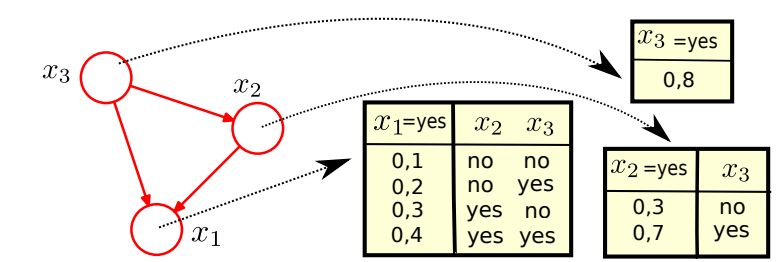
\includegraphics[width = 0.7\textwidth]{figs/bayesian-network.png}
\end{figure}

En este ejemplo, hay que completar 7 valores. Suponiendo que tenemos tres atributos binarios, habría $2^3$ combinaciones de atributos, teniendo así 8 parámetros. Como las probabilidades deben sumar 1, solo es necesario calcular 7 (siendo el último 1 - los demás). Si eliminamos las conexiones (aristas) de la red, la distribución se simplifica. Normalmente será una persona experta en los datos la cual decida qué conexiones eliminar sin impactar en los datos. De esta forma, la probabilidad de un parámetro depende de la probabilidad de su parámetro padre. 

\begin{figure}[h]
\centering
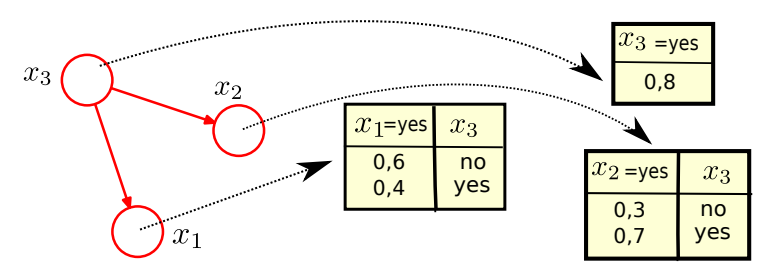
\includegraphics[width = 0.7\textwidth]{figs/bayesian-network-reduced.png}
\end{figure}

La red bayesiana de la hipótesis de Naive Bayes asume independencia, por lo que no habría ninguna arista y ningún padre. La idea sería tener algo intermedio: ni todas las aristas ni ninguna. Al quitar todas, se simplifica demasiado.

Un ejemplo para una red bayesiana sería el siguiente:
\begin{figure}[h]
\centering
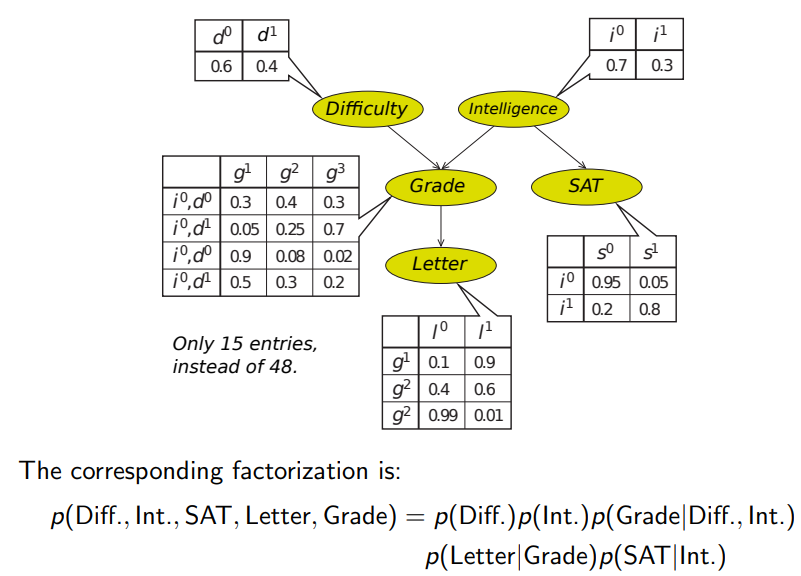
\includegraphics[width = 0.8\textwidth]{figs/bayesian-network-example.png}
\end{figure}

Con Naive Bayes tendríamos que estimar 6 valores, con la red bayesiana 15, y sin simplificación 48. Se puede utilizar una red bayesiana para obtener algo intermedio entre la hipótesis de independencia total (naive bayes) y la no simplificación.

\subsubsection{Independencia condicional}
El proceso de eliminar aristas introduce simplificaciones, las cuales son independencias condicionales. Dos variables son independientes condicionalmente si su distribución factoriza dada otra variable.
x1 es independiente de x2 dado x3, de forma que: $p(x_1, x_2 \mid x_3) = p(x_1\mid x_3) p(x_2 \mid x_3)$.

Las independencias condicionales de la distribución conjunta pueden leerse a partir del gráfico utilizando la \textbf{separación d}: Sean A, B y C conjuntos de nodos no intersecantes, entonces $A \bot B|C$ si todos los caminos desde cualquier nodo de A a cualquier nodo de B están bloqueados.
Un camino está bloqueado si contiene un nodo $n$ que o bien:
\begin{itemize}
\item las flechas se encuentran cabeza con cola o cola con cola en $n$ y $n \in C$, o
\item las flechas se encuentran cabeza con cabeza en $n$, y ni $n$, ni ninguno de sus descendientes, está en $C$.
\end{itemize}

\begin{figure}[h]
\centering
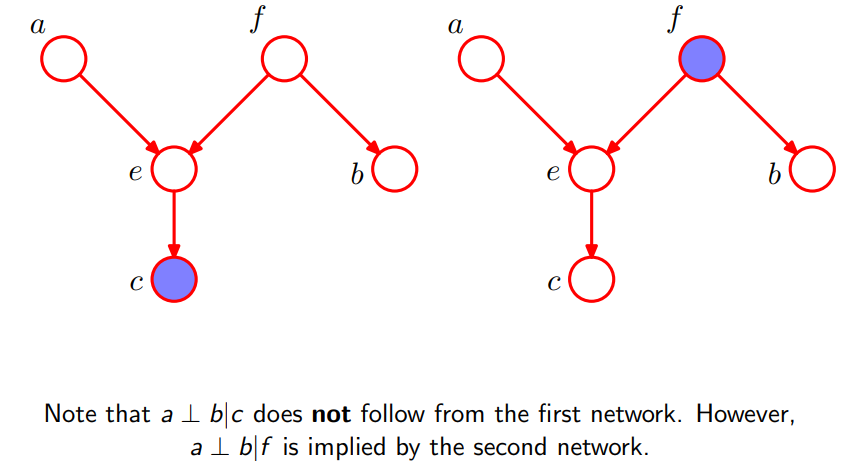
\includegraphics[width = 0.8\textwidth]{figs/conditional-independence.png}
\caption{Queremos llegar desde el nodo A al nodo B. Izquierda: se observa C, por lo que el camino no está bloqueado. No se cumple ninguno de los dos criterios anteriores, por lo que A no es independiente de B dado C, son dependientes. Esto se debe a que el nodo E tiene cabeza-con-cabeza, pero su descendiente se ha observado. Derecha: el camino de A a B está bloqueado, por lo que sí se cumple la condición y A es independiente.}
\end{figure}

El grafo bayesiano es un filtro en el que se permite el paso de $p(x)$ si y sólo si $p(x)$ satisface la propiedad de factorización dirigida. Podemos utilizar el grafo para filtrar distribuciones en función de si respetan las independencias condicionales implícitas en la separación d. El conjunto de datos final coincide entre ambos (mediante la factorización y mediante la separación).

\subsubsection{Aprendizaje en redes bayesianas}
Aprender del gráfico es muy difícil en la práctica. A menudo lo proporciona un experto con conocimientos previos sobre el proceso de generación de datos.

El aprendizaje de las tablas de probabilidad se basa en observar todas las variables, al igual que en el modelo Naive de Bayes. El aprendizaje se realiza por estimación de máxima verosimilitud o MAP. También se pueden observar solo algunas variables, pero esto requiere el uso práctico del algoritmo expectation-maximization (EM).

\subsubsection{Ejercicios}
\begin{itemize}
\item En un clasificador Naive de Bayes, $D = 5$. Los dos primeros atributos toman valores reales. El tercer atributo toma valores binarios. Los dos últimos atributos toman valores categóricos con 3 y 4 categorías diferentes. Escribe la expresión para $p(x|\mathcal{C}_k )$.

Los primeros dos factores siguen una distribución gaussiana, mientras que el restante toma una distribución de Bernoulli. 
$$p(x \mid \mathcal{C}_k) = \mathcal{N}(x_1 \mid \mu_{1k}, \sigma_{1k}^2) \mathcal{N}(x_2 \mid \mu_{2k}, \sigma_{2k}^2) p_{3k}^{x3} (1 - p_{3k})^{1-x3} \prod^3_{i = 1} \mu_{4k}^{I(x4=i)}  \prod^4_{i = 1} \mu_{5k}^{I(x5=i)}$$

\item Dada la siguiente red bayesiana, hay que buscar los caminos de x1 a x3 y si están bloqueados por x6. Es decir, hay que ver si se cumple $x_1 \bot x_3|x_6$.

\begin{figure}[h]
\centering
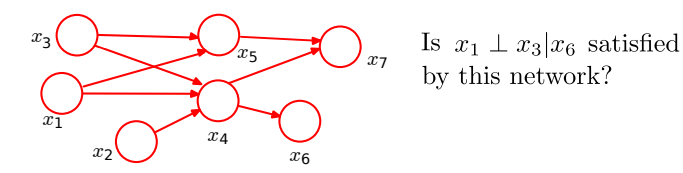
\includegraphics[width = 0.8\textwidth]{figs/bayesian-network-exercise.png}
\end{figure}

Al buscar los caminos, no nos importan los sentidos de las flechas. Los caminos son:
\begin{itemize}
\item x1-x5-x3
\item x1-x5-x7-x4-x3
\item x1-x4-x7-x5-x3
\item x1-x4-x3: no aparece x6, pero sí el padre de x6. Este padre tiene cabeza con cabeza, y como x6 está en el condicional, el camino no está bloqueado, y no podemos decir que x1 es independiente de x3 dado x6.
\end{itemize}
En el momento en que un camino no esté bloqueado, ya no podemos decir que haya independencia condicional, tienen que estar todos bloqueados.
\end{itemize}

\subsection{Resumen}
\begin{itemize}
\item Los modelos generativos de clasificación estiman $p(x|\mathcal{C}_k )$ y $p(\mathcal{C}_k )$ y utilizan el teorema de Bayes para calcular las probabilidades posteriores de clase.
\item Estimar $p(x|\mathcal{C}_k )$ puede ser un problema difícil. El clasificador Naive Bayes lo resuelve suponiendo que $p(x|\mathcal{C}_k ) = \prod^D_{j=1} p(xj |\mathcal{C}_k )$.
\item A menudo, la hipótesis del Naive Bayes no es realista y no se cumple, lo que da lugar a decisiones y resultados de clasificación subóptimos.
\item Una red bayesiana ofrece una solución intermedia (simplicidad y precisión) cuando se modela $p(x|\mathcal{C}_k )$, o cualquier otra distribución.
\item Las simplificaciones se obtienen introduciendo independencias condicionales en $p(x)$ mediante la eliminación de aristas en la red.
\end{itemize}

\section{Análisis discriminante}
Como hemos dicho antes, es poco probable que en la práctica se cumpla la hipótesis Naive de Bayes. Una red bayesiana permite simplificar este supuesto y conduce a un modelo de probabilidad más flexible cuando se trabaja con atributos categóricos. En el caso de los atributos continuos, una distribución gaussiana multivariante permite tener en cuenta las dependencias entre los atributos.

\subsection{Distribución gaussiana multivariante}
Esto permite introducir algo más flexible que la hipótesis Naive de Bayes. Las entradas de la diagonal representan la varianza de cada componente. Las entradas fuera de la diagonal son las dependencias entre variables. Si son negativas, es que existe correlación negativa entre variables. Cuando recibe el valor 0, es que no hay dependencias. 

Esto permite describir una serie de métodos para resolver problemas de clasificación: análisis discriminante. Utiliza una gaussiana multivariante para describir las condiciones multivariante. Aunque se llame análisis discriminante, se trata de un modelo generativo. Se utiliza una gaussiana para estimar las probabilidades a priori de cada clase y mediante el teorema de Bayes se puede calcular la probabilidad posterior para predecir. Si la matriz es cuadrada y la diagonal es 0, se trata de Naive Bayes. Para el prior se utilizan los estimadores de máxima verosimilitud (media empírica y promediar el vector con la media y él mismo transpuesto). 

\begin{figure}[h]
\centering
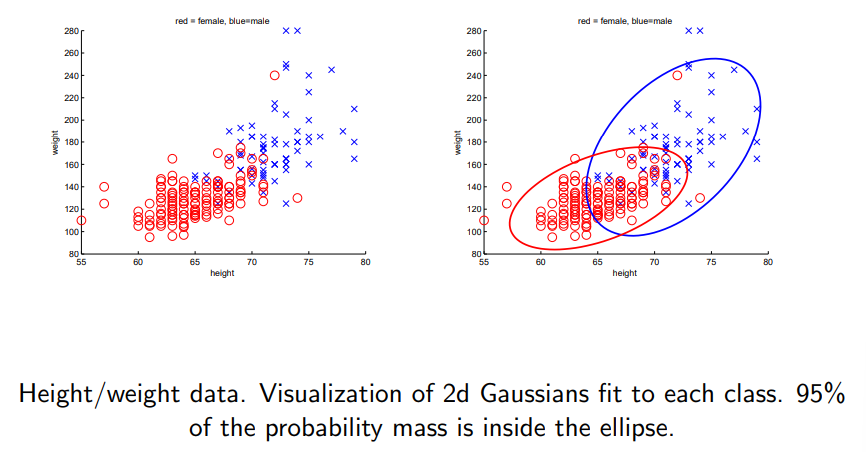
\includegraphics[width = 0.7\textwidth]{figs/multivariant-gaussian.png}
\end{figure}

\subsection{Análisis discriminante cuadrático}
Se utilizan matrices de covarianza distintas para cada clase. Al enchufar las distribuciones en la regla de Bayes, en el numerador queda el prior de la clase y la probabilidad de x dada la etiqueta de clase (densidad gaussiana multivariante). En el denominador se pone la suma del numerador para cada etiqueta de clase. 

$$
p(y_i = \mathcal{C}_k \mid \vec{x}) =
\frac{\pi_k \det(2 \pi \sigma_k)^{-1/2} \exp \left\{ -\frac{1}{2} (\vec{x} - \mu_k)^T \sigma_k^{-1} (\vec{x} - \mu_k) \right\}}
{\sum_{k'} \pi_{k'} \det(2 \pi \sigma_{k'})^{-1/2} \exp \left\{ -\frac{1}{2} (\vec{x} - \mu_{k'})^T \sigma_{k'}^{-1} (\vec{x} - \mu_{k'}) \right\} }
$$

En un problema de clasificación, la frontera está donde la probabilidad posterior para ambas clases es igual (0,5). El resultado es el análisis discriminante cuadrático, ya que la superficie de decisión es una función cuadrática (parábola).

\begin{figure}[h]
\centering
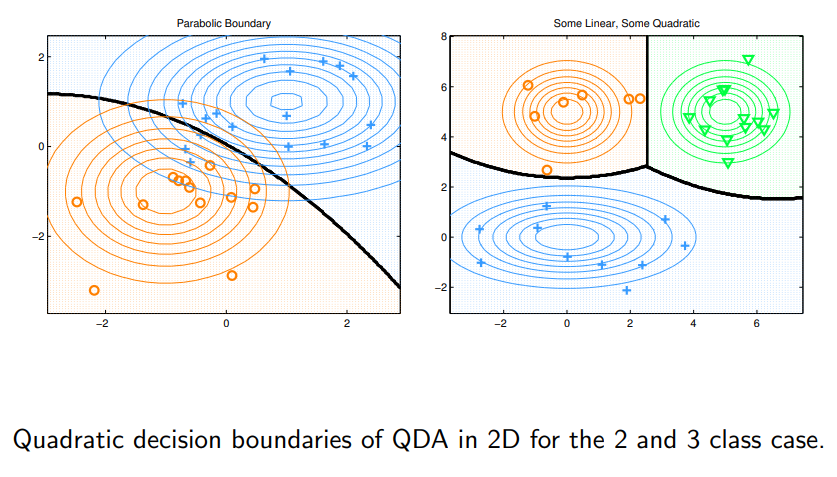
\includegraphics[width = 0.7\textwidth]{figs/qda.png}
\end{figure}

\subsection{Análisis discriminante lineal}
Cuando las matrices de covarianza para las clases se comparte (pero el vector de medias no), podemos simplificar. Así, el término cuadrático que depende de x por la matriz de covarianza invertida por x, se puede meter en un término constante. La frontera de clasificación va a ser lineal.

\begin{figure}[h]
\centering
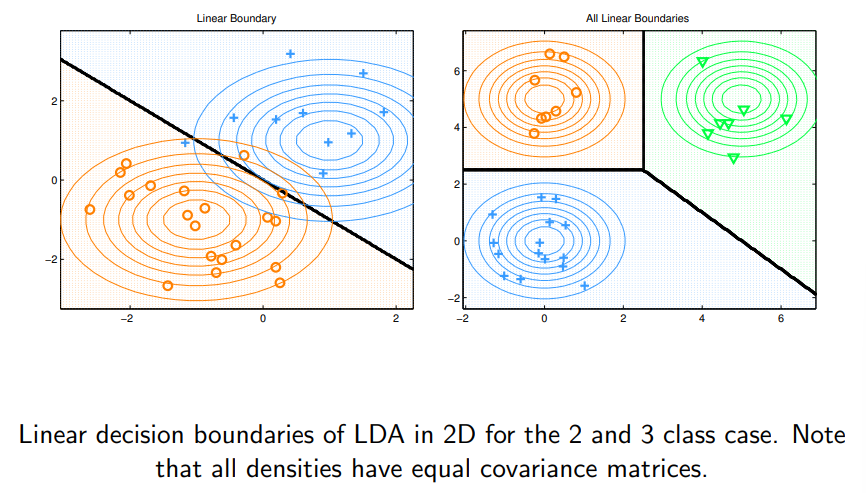
\includegraphics[width = 0.7\textwidth]{figs/lda.png}
\end{figure}

Lo difícil de este método es estimar las matrices de covarianza. Para ello, se maximiza la probabilidad de los datos observados, donde la media depende de la etiqueta de clase de donde venga. Se puede utilizar el estimador de máxima verosimilitud, quedando una mezcla de la máxima verosimilitud para las dos gaussianas.

Entre estos dos análisis (el cuadrático y el lineal), es el cuadrático el que tiene más términos y también el más flexible. Además, el cuadrático es el que tiene mayor riesgo de sobreajuste. El lineal es más robusto: tiene menos parámetros, es menos flexible, pero tiene menos riesgo de sobreajustar a los datos de entrenamiento.

%24/03 - Daniel Hernández
La única diferencia entre los dos análisis es la estimación de la matriz de covarianza (para el cuadrático hay dos matrices, para el lineal es compartida entre las clases). Hay que maximizar la matriz de covarianza observada con respecto a la matriz sigma. Se obtiene el estimador de máxima verosmilitud para la matriz de covarianza, siendo el promedio de las matrices de covarianzas de las distintas etiquetas de clase. 

\subsubsection{Sobreaprendizaje}
El análisis discriminante cuadrático es más sensible al sobreaprendizaje, pudiendo haber problemas cuando hay pocos datos. A la hora de calcular las probabilidades posteriores de clase, hay que calcular las inversas de las matrices de covarianza. Si el número de datos es menor que el de las observaciones, no va a ser posible la inversión, siendo un problema para estos clasificadores. Si ocurre eso, la matriz de covarianza no se puede invertir, por lo que se hace diagonal. En ese caso, iríamos al clasificador de Naive Bayes. Otra técnica podría ser igualar todas las matrices de covarianza, juntando los datos de todas las clases, aplicando el análisis discriminante lineal. Alternativamente, se puede forzar que las matrices de covarianza sean iguales y forzar que sean diagonales, utilizando el clasificador del análisis discriminante lineal diagonal. Por último, se puede utilizar la estimación máxima a posteriori para ajustar la matriz de covarianza. 

\subsection{Análisis discriminante regularizado (RDA)}
Se puede introducir como prior para la matriz de covarianzas la distribución de probabilidad de Wishart. Tiene dos parámetros: la media de la distribución (una matriz de covarianzas alrededor de la que estarían nuestras matrices) y un escalar que define la dispersión alrededor de la media. Con esta distribución definimos que esperamos que la matriz de covarianzas esté cerca de la matriz de identidad. El parámetro de dispersión es equivalente a $\lambda$, que afectaría al parámetro máximo a posteriori. $\lambda$ tomaría valores entre 0 y 1, mientras que MAP sería una combinación entre la matriz prior y máxima verosimilitud. Lo ideal sería poner algo intermedio entre los dos valores. Para algunos valores de $\lambda$ podemos obtener algunas matrices invertibles, mejores que las de MAP. Esto introduce un hiperparámetro al modelo que se debe ajustar. Para ello, se utilizan técnicas de comparación de modelos mediante la validación cruzada. 

Hay que tener cuidado a la hora de elegir hiperparámetros. Cuando se ajusta, no se pueden utilizar datos de tests, ya que se utilizarían para construir el clasificador y ya no sería independiente a ellos. La estimación sería sesgada. Para ajustar los hiperparámetros, se haría validación cruzada sobre los datos de entrenamiento. Se obtendría el valor de $\lambda$ con el que funcione mejor el modelo y se evalúa con los datos de test.

\subsection{Análisis discriminante lineal diagonal}
En el caso de que la matriz de covarianza sea diagonal y compartida entre todas las clases, se conoce el modelo como análisis discriminante lineal diagonal. Para cuando hay muchas dimensiones, esto funciona mejor que otros análisis. Esto es menos flexible al tener menos parámetros, por lo que es bueno con pocos datos de entrenamiento y muchas dimensiones, ya que se limita el riesgo de sobreaprendizaje.

\subsection{Clasificador Nearest Shrunken Centroids}
Este clasificador es una variante del anterior en el que solo algunos atributos son relevantes. En lugar de hacer estimación máxima a posteriori para la matriz, se utiliza MAP para las medias. La media de cada clase es igual a una media común igual para todas las clases y un término diferenciador que va a ser el que diferencie las etiquetas de clase. A eso se le conoce como centroide. Se fuerza que ese término se aproxime a 0. Cuando el término se hace exactamente a 0, la media para todas las clases es la misma, siendo la media para ese atributo. Esto se traduce en que el atributo es irrelevante para calcular la probabilidad a posteriori, al contribuir de la misma manera para cada una de las distintas etiquetas de clase, sin introducir ningún cambio en el cálculo de las probabilidades posteriores. Así, se hace una selección de atributos. 

Para que los centroides se aproximen a 0, hay un hiperparámetro entre 0 y el máximo valor de los centroides, siendo esa la cantidad que se sustrae a los centroides. Si se sustituye para que los centroides sean 0, lo que queda es el prior en la regla de Bayes. 

Este clasificador tiene un hiperparámetro que indica lo que se encogen los centroides. Si no se encogen, tenemos un análisis discriminante lineal, y si se encogen mucho, el prior de las clases. Por ello, se debe estimar el hiperparámetro con validación cruzada.  

\subsection{Ejercicios}
\begin{enumerate}
\item ¿Qué ventajas y desventajas tienen QDA y LDA?

QDA tiene fronteras más flexibles al ser parábolas en comparación con las fronteras lineales de LDA. No obstante, es más propenso al sobreaprendizaje con un peor error de generalización.

\item Imagina que aplicas QDA a un problema de clasificación con más atributos que datos. La matriz es singular y no inversa. ¿Qué técnicas se pueden utilizar para resolver este problema?

Se puede utilizar la estimación máxima a posteriori y ajustar $\lambda$ que interpola entre una matriz igual a la de identidad y una matriz diagonal. Esta es una de las soluciones. Otra solución sería coger la diagonal, quedando así Naive Bayes. También se podrían forzar las matrices de covarianza para que fueran iguales (y por tanto, compartidas).
\end{enumerate}

\subsection{Resumen}
\begin{itemize}
\item Es poco probable que se cumpla la hipótesis Naive Bayes. Una distribución gaussiana multivariante puede tener en cuenta las dependencias.
\item El análisis discriminante surge utilizando el teorema de Bayes y una gaussiana multivariante para estimar las densidades condicionales de clase.
\item QDA considera diferentes matrices de covarianza para cada densidad condicional de clase, que pueden estimarse utilizando ML. Los límites de decisión de QDA son funciones cuadráticas.
\item LDA considera matrices de covarianza compartidas para cada densidad condicional de clase. Los límites de decisión de LDA son funciones lineales. Es menos flexible pero más robusto al sobreajuste.
\item DLDA es una variante de LDA que asume una matriz de covarianza diagonal.
\item Para mejorar la robustez de los métodos discriminantes se puede utilizar la estimación MAP. En algunos casos, esto conduce a la selección de atributos.
\end{itemize}

\section{Vecinos próximos y árboles de clasificación}
\subsection{Vecinos más próximos y estimación de la densidad}
Hasta ahora, hemos creado modelos generativos con probabilidades condicionales calculadas con el teorema de Bayes para hacer predicciones. Calcular las estimaciones condicionales es complicado de hacer en la práctica. 

La hipótesis de gaussianidad es restrictiva al ser unimodal, lo cual no siempre coincide. Los vecinos próximos es más flexible que la distribución gaussiana. Se estiman densidades de distribuciones (cada etiqueta de clase). La probabilidad de que los datos caigan en una región en el espacio depende del área bajo la curva de la densidad. 

Imaginemos que tenemos datos observados, teniendo que estimar la densidad de probabilidad en dos regiones. La probabilidad de que los datos caigan en la región 1 es el área debajo de la curva de la densidad de la región 1. 

\begin{figure}[h]
\centering
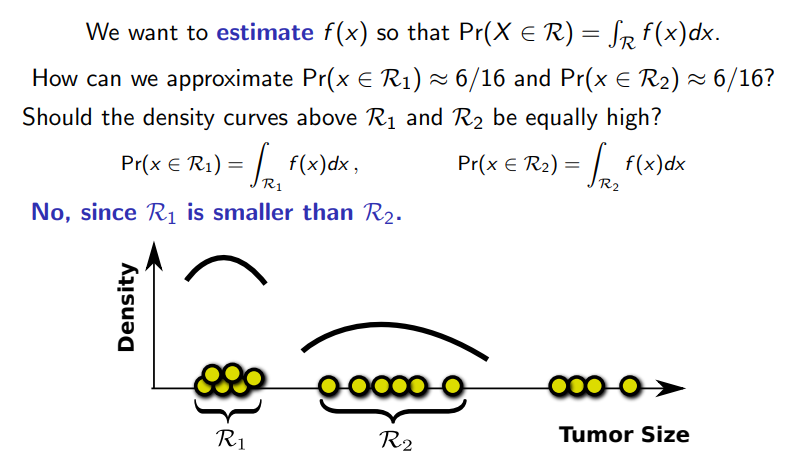
\includegraphics[width = 0.8\textwidth]{figs/density-estimation.png}
\end{figure}

La estimación de densidad se debe normalizar en cuanto al tamaño de la región. Suponemos que la densidades son constantes (que la curva es plana), el área bajo la curva es un rectángulo, altura por longitud, es decir, densidad de probabilidad por anchura de la región.

De esta forma, la densidad se puede aproximar como:
$$f(x) \approx \frac{\text{number of samples in region}}{\text{total number of samples}} \cdot \frac{1}{\text{volume of the region}} = \frac{\kappa}{N} \frac{1}{V}$$

Esto se debe estimar para cada etiqueta de clase. Si hacemos esto, para la estimación de la distribución condicional queda:
$$p(\vec{x} \mid \mathcal{C}_k) \approx \frac{N_k(\vec{x})}{N_k V(\vec{x})}$$
Este estimador es para la distribución condicional, y se utiliza en la regla de Bayes para las probabilidades posteriores:
$$p(y_i = \mathcal{C}_k \mid \vec{x}) = \frac{N_k (\vec{x})}{\sum_{k'} N_{k'}(\vec{x})} = \frac{N_k(\vec{x})}{\kappa}$$

Así, en la clasificación de vecinos $\kappa$-próximos, simplemente hay que predecir la clase más común entre los $\kappa$ vecinos de x. Una $\kappa$ pequeña produce muchas regiones pequeñas de cada clase, mientras que una $\kappa$ grande da lugar a menos regiones grandes.

Las ventajas de este clasificador son:
\begin{itemize}
\item Puede aplicarse a los datos de cualquier distribución.
\item Muy sencillo e intuitivo.
\item No paramétrico: más expresivo a medida que tenemos más muestras.
\item Buen rendimiento si el número de muestras es grande.
\end{itemize}

No obstante, también tiene algunas desventajas:
\begin{itemize}
\item Elegir el mejor $\kappa$ puede ser difícil, realizándose mediante búsqueda en validación cruzada. Una $\kappa$ pequeña provoca un sobreajuste, y una $\kappa$ pequeña un infraajuste.
\item Es computacionalmente pesado al necesitar almacenar todos los datos de entrenamiento.
\item Se necesita un gran número de muestras para obtener una buena precisión.
\end{itemize}

\subsection{Árboles de clasificación}
Es natural clasificar un patrón mediante una secuencia de preguntas, en la que la siguiente pregunta depende de la respuesta a la pregunta actual. La principal ventaja es la interpretabilidad. Es sencillo transformar el árbol en un conjunto de reglas de clasificación.

\begin{figure}[h]
\centering
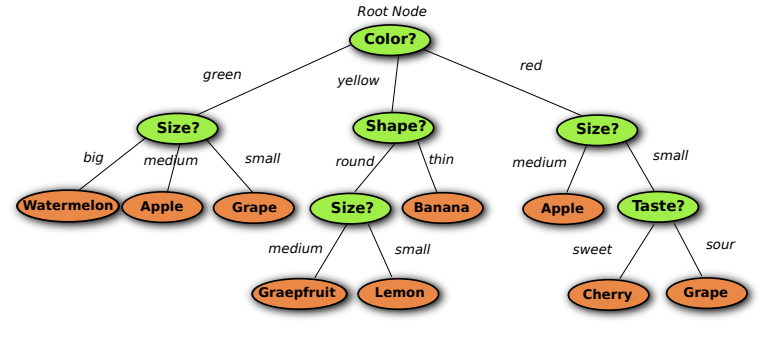
\includegraphics[width = 0.8\textwidth]{figs/classification-tree.png}
\end{figure}

El aprendizaje de árboles de decisión suele ser más adecuado si
\begin{itemize}
\item Varios atributos categóricos, por ejemplo, el tamaño puede ser pequeño, mediano o grande.
\item El problema de clasificación tiene varias etiquetas, es decir, es multiclase.
\item Los datos de entrenamiento pueden contener errores (atributos o etiquetas).
\item Los datos de entrenamiento pueden contener valores perdidos (missing values).
\item Nos interesa la interpretabilidad del clasificador.
\end{itemize}

La mayoría de los algoritmos emplean una búsqueda codiciosa descendente:
\begin{enumerate}
\item Se determina qué atributo debe comprobarse en la raíz.
\item A continuación, se crean descendientes para cada valor posible.
\item Los datos de entrenamiento se clasifican en el descendiente apropiado.
\item El proceso se repite con los datos asociados a cada descendiente.
\item El proceso se detiene, por ejemplo, cuando todos los casos pertenecen a la misma clase.
\end{enumerate}

\begin{figure}[h]
\centering
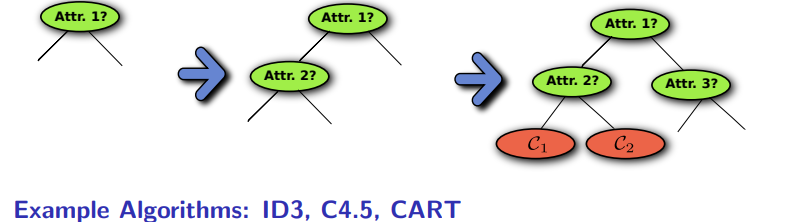
\includegraphics[width = 0.8\textwidth]{figs/tree-construction.png}
\end{figure}

\subsubsection{Selección de test en cada nodo}
¿Qué atributo debemos seleccionar en cada nodo? La idea clave es seleccionar el atributo que sea más útil para clasificar. Esto dará lugar a árboles más pequeños y compactos, y requiere una medida de impureza de los datos. Esta impureza se mide con la entropía, el índice de Gini o la tasa de error. Todas las medidas son altas en el 50\% de cada clase.

Dada una determinada medida de impureza, ¿qué atributo debemos seleccionar para dividir en el nodo del árbol parcial? Una heurística elige el atributo que disminuye más la impureza. Se trata de una regla codiciosa que intenta generar árboles pequeños.

Como ejemplo, retomamos el dataset de la clasificación tumoral (con size, smoothness y symmetry). Utilizando la entropía, hay 5 ejemplos de la clase positiva y 9 de la negativa. La impureza de los datos es la entropía de un conjunto de datos con 9 ejemplos de la clase negativa y 5 de la positiva. Los cálculos serían
$$5/9 \cdot  log_2(5/14) - 9/14 \cdot log_2(9/14) = 0.940286$$

Ahora queremos ver la reducción esperada de la impureza de los datos al utilizar el atributo symmetry para separar los datos. Es un atributo binario con 6 datos yes y 8 no. De los 6, hay 5 ejemplos de la clase negativa y 1 de la positiva, mientras que de los 8 son 4 de la clase positiva y 4 de la negativa. Así:
$$0.94 - 6/14 log_2(6/14) - 8/14 log_2(8/14) = 0.09$$

Ahora consideramos el tamaño:
$$0.94 - 5/14 log_2(5/14) - 5/14 log_2(5/14) - 4/14 \cdot 0 = 0.424$$

Comparando los dos resultados, la entropía de tamaño es mayor, por lo que es un mejor atributo para la raíz. También habría que tener en cuenta smoothness para determinar la raíz. Los resultados son:
\begin{itemize}
\item Smoothness = 0.119
\item Symmetry = 0.09
\item Size = 0.424
\end{itemize}

La mayor disminución de la impureza de los datos corresponde a Tamaño. El nodo raíz comprueba el atributo Tamaño y el proceso se repite para cada hijo hasta que se cumple un criterio de parada.

\begin{figure}[h]
\centering
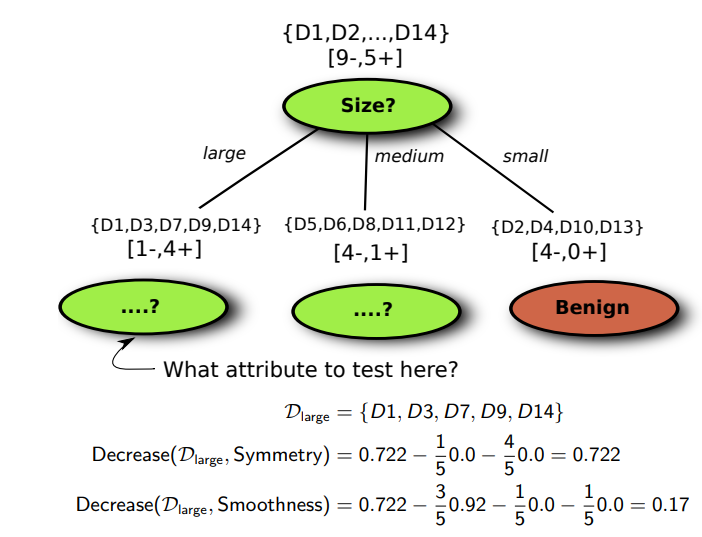
\includegraphics[width = 0.8\textwidth]{figs/tree-result.png}
\end{figure}

\subsubsection{Tamaño del árbol}
Si el tamaño del árbol es muy grande, puede ajustarse en exceso a los datos. Por el contrario, si el tamaño es demasiado pequeño, puede no ajustarse lo suficiente a los datos.
Existen diferentes métodos para evitar que crezcan árboles demasiado grandes:
\begin{itemize}
\item Mantener un conjunto de validación (10\% de los datos). Continúa dividiendo nodos hasta que se minimice el error en los datos de validación.
\item La división se detiene si la mejor división reduce la impureza en menos de una cantidad preestablecida $\beta$, es decir, si $max_a Decrease(\mathcal{D}, a) \leq \beta$.
\item Se detiene cuando un nodo tiene menos de algún número umbral de puntos$N_{min}$ o algún porcentaje del conjunto total de entrenamiento, por ejemplo, 5\%.
\item Intercambia complejidad por precisión de la prueba
\end{itemize}

\subsubsection{Estrategias post-pruning}
La división detenida adolece de falta de suficiente visión de futuro, por lo que es preferible la realizar post-pruning.

Hay que hacer crecer un árbol hasta que los nodos de las hojas tengan una impureza mínima. A continuación, se considera cada nodo del árbol como candidato a la poda:
\begin{itemize}
\item Eliminar el subárbol completo enraizado en ese nodo.
\item Convertir el nodo eliminado en una hoja.
\item Asignar la clase más común dentro de los datos que llegan a ese nodo.
\end{itemize}

Los nodos se podan de forma iterativa, eligiendo el nodo cuya eliminación más aumenta la precisión en el conjunto de validación. La poda continúa hasta que una nueva poda resulte perjudicial.

\subsubsection{Incorporación de atributos continuos}
Se ordenan los atributos continuos de menor a mayor y se observa en qué rango hay un cambio de la etiqueta.

\subsection{Resumen}
\begin{itemize}
\item Los vecinos más próximos son un método de clasificación no paramétrico muy sencillo cuya capacidad expresiva crece con el tamaño del conjunto de datos.
\item El número de vecinos $\kappa$ especifica la complejidad del modelo. Un valor alto de $\kappa$ conduce a un ajuste insuficiente y $\kappa$ pequeño conduce a un ajuste excesivo.
\item Los árboles son modelos interpretables que dividen los datos en cada nodo. Tratan atributos continuos, categóricos y ausentes.
\item Los árboles se generan mediante un algoritmo codicioso que trata de encontrar la mejor división en cada nodo para reducir al máximo la impureza de los datos.
\item Los árboles completamente desarrollados suelen ajustarse en exceso a los datos de entrenamiento, por lo que las estrategias de poda a posteriori, en las que se reduce el tamaño del árbol, son necesarias. 
\item Los árboles de clasificación tienden a funcionar un poco peor que otros modelos.
\end{itemize} 

%25/03 - Daniel Hernández
\section{Combinación de clasificadores: métodos ensemble}
La predicción del conjunto de los clasificadores individuales será la clase mayoritaria. De esta forma, se puede probar si los errores de los clasificadores son independientes, teniendo así una clasificación mejorada. 

\begin{figure}[h]
\centering
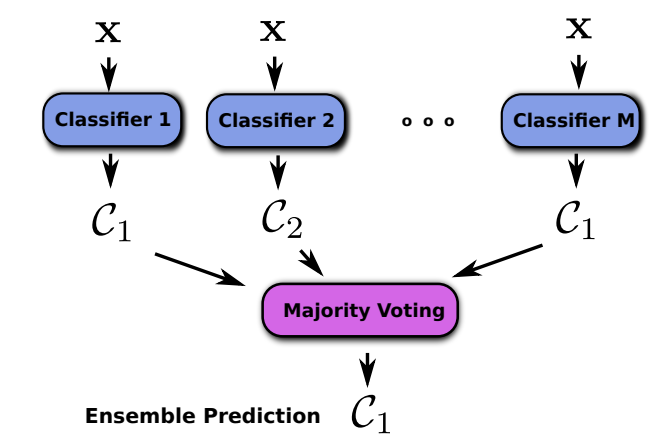
\includegraphics[width = 0.6\textwidth]{figs/majority-voting.png}
\end{figure}

El ensemble puede reducir significativamente el error de un único clasificador simplemente considerando varias versiones del mismo. Por desgracia, los errores cometidos por los clasificadores no son independientes en la práctica. Sólo existe un único conjunto de datos de entrenamiento D, y hay que introducir variabilidad entre los clasificadores utilizando diferentes técnicas:
\begin{itemize}
\item Entrenamiento de cada clasificador en una muestra bootstrap.
\item Inyección de ruido en el conjunto de entrenamiento (cambiar algunas etiquetas).
\item Introduciendo cierta aleatoriedad en el algoritmo de entrenamiento.
\end{itemize}

Los errores suelen estar sólo ligeramente correlacionados, y la reducción del error global suele ser significativa.

\subsection{Bagging, agregación de bootstrap}
Cada clasificador base se entrena en una muestra bootstrap de los datos, y se utiliza la votación por mayoría para combinar los resultados de los clasificadores. Al construir una muestra bootstrap, se pueden repetir algunos datos en una misma muestra, y algunos datos pueden faltar. En torno a un tercio de los datos de una muestra de bootstrap van a estar repetidos, y por tanto en torno a un tercio de los datos totales no van a estar presentes. 

\begin{figure}[h]
\centering
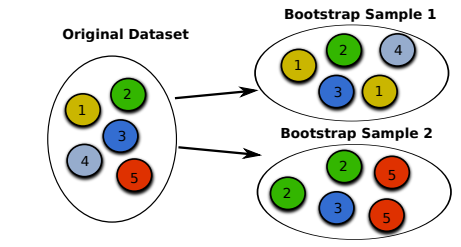
\includegraphics[width = 0.6\textwidth]{figs/bootstrap.png}
\end{figure}

Las características del Bagging son:
\begin{itemize}
\item Puede aplicarse a cualquier algoritmo de clasificación (normalmente árboles).
\item El error de un clasificador suele ser mayor (debido al muestreo bootstrap).
\item El error del conjunto disminuye con M y suele ser mucho mejor.
\item Funciona mejor con clasificadores inestables (reduce la varianza). Estos clasificadores tienen grandes cambios en los límites de decisión y la predicción con pequeños cambios en el conjunto de entrenamiento. Por ejemplo, los árboles de clasificación no podados serían un clasificador inestable.
\item Puede degradar el rendimiento de los clasificadores estables, es decir, clasificadores en los cuales grandes cambios en el conjunto de entrenamiento producen pequeños en los límites de decisión (predicciones), como pueden ser los K-vecinos más próximos.
\end{itemize}

El bagging es peor al principio que utilizar un solo clasificador debido al bootstrap (se utilizarían menos datos de entrenamiento), pero al final es mejor que un solo árbol. No obstante, es más costoso computacionalmente, ya que hay que generar varios clasificadores. Otra desventaja es que la interpretabilidad se pierde, pero al menos se mejora el error de clasificación. 

\subsection{Cambio de clases}
Cada clasificador base se entrena en una versión corrupta de los datos. Cada vez, se cambia aleatoriamente la etiqueta de una fracción p de los datos. Se utiliza la votación por mayoría para combinar los resultados de los clasificadores.

\begin{figure}[h]
\centering
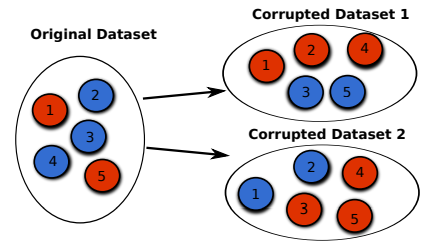
\includegraphics[width = 0.6\textwidth]{figs/class-switching.png}
\end{figure}

Este cambio de clase obliga a cometer errores independientes de forma más agresiva que el bagging. Requiere ajustar un (hiper)parámetro adicional p que depende del problema. A menudo se requieren conjuntos de mayor tamaño que en el bagging. Un p grande tiende a funcionar mejor, pero también requiere valores más grandes de M. 

\begin{figure}[h]
\centering
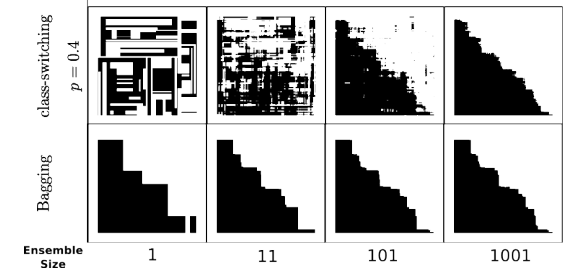
\includegraphics[width = 0.7\textwidth]{figs/bagging-classswitching.png}
\end{figure}

Comparando el cambio de clases con el uso de un solo clasificador y el bagging, al principio es el peor método, pero al final es el mejor.

\begin{figure}[h]
\centering
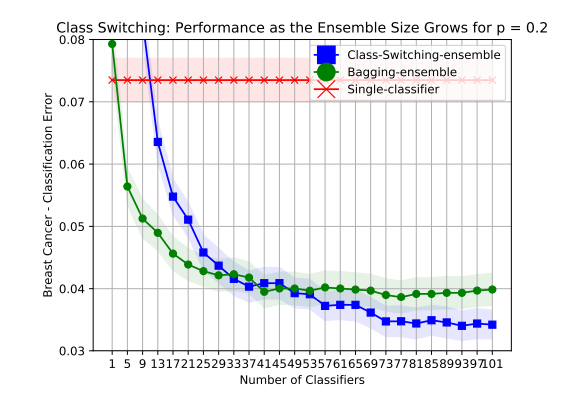
\includegraphics[width = 0.7\textwidth]{figs/noclass-bagging-classswitching.png}
\end{figure}

Cuando p aumenta, el error del conjunto tarda más en converger, por lo que pueden ser necesarios conjuntos más grandes.

\subsection{Random forest}
Cada clasificador de árbol se entrena en una muestra bootstrap de los datos. Se introduce una cierta aleatoriedad en el algoritmo de crecimiento de los árboles, y se permite que éstos crezcan al completo, sin poda. Se utiliza la votación por mayoría para combinar los resultados de los clasificadores. 

La aleatoriedad se introduce en el proceso de crecimiento del árbol:
\begin{itemize}
\item En cada nodo, se elige un subconjunto aleatorio de m < D atributos.
\item Se calcula la disminución de impurezas para cada uno de los m atributos.
\item Se dividen los datos en ese nodo utilizando el atributo con la mayor disminución.
\end{itemize}

Este proceso introduce variabilidad en los clasificadores y decorrelaciona los errores cometidos.

\begin{figure}[h]
\centering
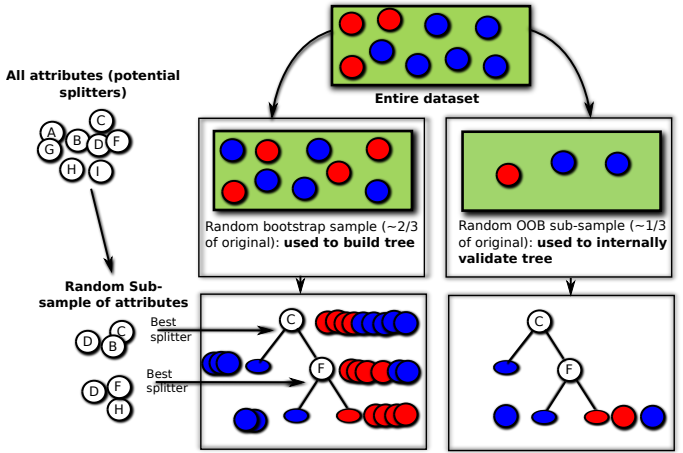
\includegraphics[width = 0.6\textwidth]{figs/random-forest-indv.png}
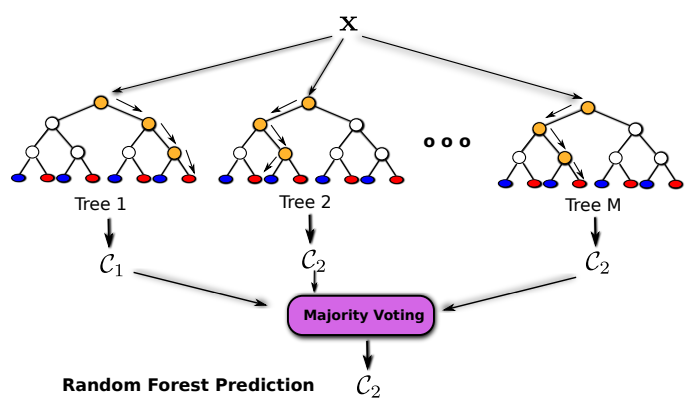
\includegraphics[width = 0.6\textwidth]{figs/random-forest-prediction.png}
\end{figure}

Random forest es más eficaz que bagging a la hora de generar árboles diversos. El proceso de construcción de cada árbol es más rápido, y debido a la aleatorización de las divisiones, los árboles son más grandes. Los datos fuera de bootstrap (OOB) se utilizan para estimar el error de prueba de forma gratuita. Además, es bastante insensible al parámetro m (a menudo, $m = \sqrt{D}$).

\begin{figure}[h]
\centering
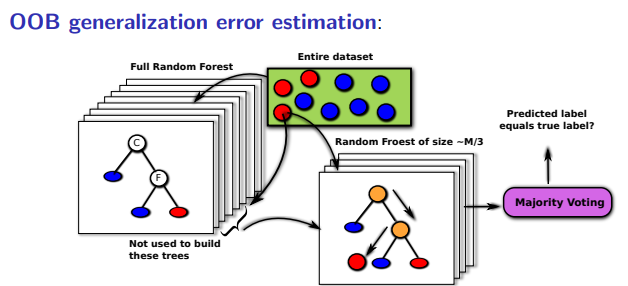
\includegraphics[width = 0.6\textwidth]{figs/random-forest-error.png}
\end{figure}

Random forest ofrece mejores resultados que el bagging y el árbol único.

\begin{figure}[h]
\centering
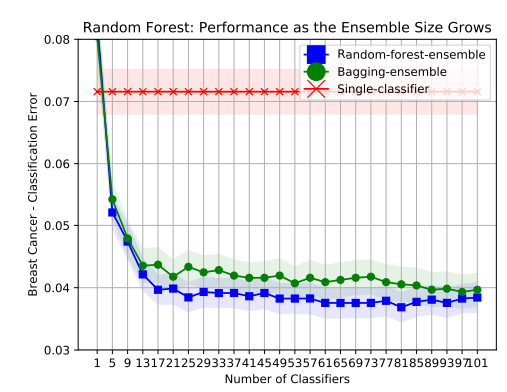
\includegraphics[width = 0.7\textwidth]{figs/noclass-bagging-randomforest.png}
\end{figure}

\subsection{Resumen}
\begin{itemize}
\item Los métodos de ensamblaje pueden mejorar significativamente el rendimiento de un clasificador base, aunque pueden reducir la interpretabilidad.
\item Un buen ensemble debe contener clasificadores que cometan errores independientes pero que también sean relativamente precisos (mejores que los aleatorios).
\item El bagging introduce diversidad en los clasificadores de base mediante el ajuste de cada clasificador a una muestra bootstrap de los datos.
\item El cambio de clase invierte aleatoriamente las etiquetas de los datos.
\item El random forest añade más aleatoriedad al proceso de crecimiento del árbol.
\end{itemize}

El método por defecto basado en conjuntos de clasificadores es random forest.

\section{Selección de atributos}
La selección de atributos se realiza con técnicas que identifican unos pocos atributos relevantes del conjunto total de atributos que son más útiles para abordar una tarea de clasificación. También se denomina como selección de variables o selección de atributos. Es diferente a las técnicas de extracción de características, que crean nuevas características a partir de funciones de las características originales, como por ejemplo: PCA.

\begin{figure}[h]
\centering
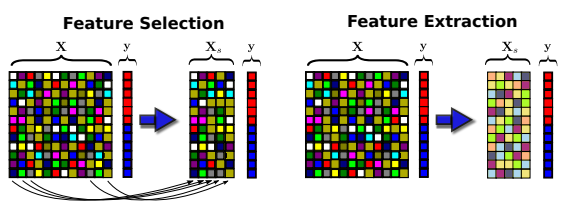
\includegraphics[width = 0.7\textwidth]{figs/feature-selection-extraction.png}
\end{figure}

La selección de atributos se realiza por los siguientes motivos:
\begin{itemize}
\item Simplificación de los clasificadores para facilitar su interpretación.
\item Tiempos de entrenamiento más cortos.
\item Aliviar la maldición de la dimensionalidad.
\item Mejorar la generalización reduciendo el sobreajuste.
\item Simplificar la recogida de datos.
\end{itemize}

En las técnicas de selección de rasgos, el objetivo es identificar qué rasgos son
\begin{itemize}
\item \textbf{Relevantes:} Características que son estrictamente necesarias para obtener buenos resultados en la tarea de predicción. Sin ellas, el error de generalización aumenta.
\item \textbf{Irrelevantes:} Características innecesarias para la tarea de clasificación. El error de generalización no se reduce al considerarlas.
\item \textbf{Redundantes:} Características que se vuelven irrelevantes en presencia de otras características relevantes para la clasificación.
\end{itemize}

El objetivo de las técnicas de selección de características es identificar las características relevantes y excluir las irrelevantes y redundantes.

Hay dos posibles escenarios que pueden surgir: 
\begin{enumerate}
\item \textbf{Gran número de datos, pero con pocas dimensiones/atributos:} al utilizar un método de selección de atributos, en esta situación va a ayudar algo, pero no demasiado a la hora de mejorar el error de clasificación. 
\item \textbf{Número pequeño de datos y muchas dimensiones:} en este escenario, la selección de atributos será clave. Esto se puede dar en estudios clínicos con pocos pacientes, pero muchos genes de los que se mide la expresión. La selección de atributos puede ser interesante para identificar un número reducido de genes que sean relevantes para predecir la enfermedad, obteniendo un subset interpretable que ayude a los médicos.
\end{enumerate}

En función del número de variables consideradas conjuntamente, se distinguen:
\begin{itemize}
\item \textbf{Métodos univariantes, clasificación de variables}: Consideran las variables de entrada una a una. Puede ignorar variables importantes.
\item \textbf{Métodos multivariantes, selección de subconjuntos de variables}: considera grupos de variables juntos. No es posible probar todas las combinaciones
\end{itemize}

Basado en el uso de un clasificador en la selección de características:
\begin{itemize}
\item \textbf{Filtro}: selecciona un subconjunto de variables independientemente del clasificador que luego las utilizará. A menudo, métodos univariantes.
\item \textbf{Wrapper}: selecciona un subconjunto de variables teniendo en cuenta la precisión del clasificador que las utilizará.
\item \textbf{Embebido}: el método de selección de características se incorpora al proceso de entrenamiento del clasificador (por ejemplo, árboles de clasificación o centroides encogidos).
\end{itemize}

\subsection{Métodos de filtrado}
Este método se basa en encontrar un subconjunto de variables de las que se espera un buen rendimiento utilizando únicamente los datos observados X e y. En el \textbf{ranking de variables}, se calcula el estadístico J para cada atributo y se mantienen los valores por encima de un umbral. Este método es univariable al mirarse cada atributo de forma individual.

Uno de los scores que se puede utilizar en variable ranking es ANOVA. Se realiza el análisis de la varianza como prueba estadística para evaluar si las medias de varios grupos son iguales o no. Se obtiene el F-score. F será grande si la variabilidad entre grupos es grande en relación con la variabilidad dentro de los grupos (poco probable si todas las medias son iguales).

La ventaja de los filtros es que son rápidos de computar, y permite la selección genérica de variables sin estar condicionado por ningún clasificador. Requiere un paso de preprocesado para reducir el espacio de dimensionalidad y el sobreajuste. No obstante, filtros simples pueden ignorar variables que solo son relevantes en conjunto con otras.

\subsection{Wrappers}
Los wrappers permiten evaluar la calidad de un subconjunto de características en función de la precisión de un clasificador concreto. Implica evaluar muchos subconjuntos diferentes. Es un proceso interativo en el que, en cada iteración, se generan y evalúan varios subconjuntos de atributos. El éxito de cada subconjunto determina qué subconjuntos se probarán a continuación. La selección de características pasa a formar parte del entrenamiento del clasificador.

La ventaja es que puede utilizarse con cualquier clasificador, y la selección de variables está sintonizada para un clasificador dado. Además, puede encontrar atributos que sean relevantes conjuntamente. No obstante, es muy costoso computacionalmente, y requiere dejar de lado los datos de validación.
Las características D dan $2^D$ posibles subconjuntos, por lo que es necesario una estrategia de búsqueda: selección secuencial hacia delante, eliminación recursiva hacia atrás, algoritmos genéticos, annealing simulado, etc.

\subsection{Métodos embebidos}
En este caso, el proceso de selección de características se realiza durante el entrenamiento del clasificador. Ejemplos son árboles de decisión, centroides encogidos más próximos o LASSO generalizado. Este último es un modelo discriminativo que contiene el hiperparámetro w. 

La selección de variables se realiza de forma gratuita mientras se entrena el clasificador. De esta forma, pueden encontrarse atributos que sean relevantes conjuntamente y utilizar conocimientos sobre el algoritmo de clasificación específico. Además, suele ser más barato que los métodos wrappers y tiene un buen rendimiento empírico en general. La desventaja es que suele requerir el ajuste de hiperparámetros mediante validación cruzada, y las características seleccionadas son específicas del clasificador. 

\subsection{Medidas de dependencia: correlación lineal}
Es importante medir la dependencia de un atributo con la etiqueta de clase. Si las dependencias son grandes, es bastante probable que el atributo sea relevante. 

La correlación entre dos variables toma valores entre -1 y 1. Esos valores indican que la dependencia es fuerte. El coeficiente al cuadrado toma valores entre 0 y 1, e indica así la fracción de varianza total que se explica mediante una relación lineal simple entre el atributo y la etiqueta de clase. 

\begin{figure}[h]
\centering
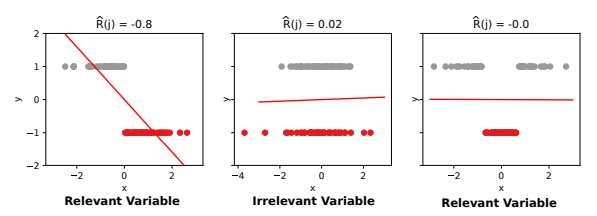
\includegraphics[width = 0.7\textwidth]{figs/linear-correlation.png}
\end{figure}

La correlación lineal solo tiene sentido en problemas de clasificación cuando el problema es binario. Además, solo puede captar las dependencias lineales y puede subestimar variables importantes. 

\subsection{Medidas de dependencia: información mutua}
La información mutua mide la información que comparten x e y: En qué medida el conocimiento de una de estas variables reduce la incertidumbre sobre la otra. Esto se puede definir de muchas formas, entre las que se incluye la entropía.

La entropía condicional es la incertidumbre en y después de conocer x.

\begin{figure}[h]
\centering
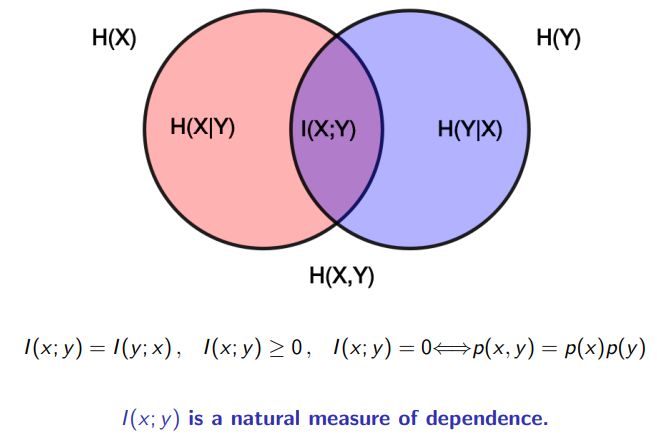
\includegraphics[width = 0.7\textwidth]{figs/mutual-information.png}
\end{figure}

En la práctica, $I(x;y)$ capta las dependencias no lineales, a diferencia de la correlación lineal. $y$ no tiene por qué ser binario (asignado a un conjunto entero). En el caso discreto, I(x; y) puede estimarse simplemente contando. En el caso continuo, es necesario estimar la densidad (muy difícil). A menudo, las variables se discretizan o se utilizan técnicas basadas en los vecinos más próximos para su estimación.

\begin{figure}[h]
\centering
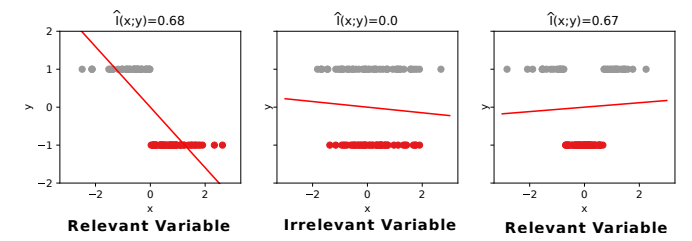
\includegraphics[width = 0.7\textwidth]{figs/mutual-information-practice.png}
\end{figure}

\subsection{Métodos de filtrado avanzado}
Un enfoque heurístico común es una búsqueda secuencial que considera las características una por una para añadirlas/eliminarlas.
Dos enfoques secuenciales populares son:
\begin{itemize}
\item \textbf{Selección hacia delante:} añade la característica que maximiza $J(x., j)$
\item \textbf{Eliminación hacia atrás:} elimina la característica que minimiza J.
\end{itemize}

\subsubsection{Minimum-Redundancy Maximum-Relevance}
Éste es un criterio que favorece las características relevantes que no son redundantes
$$J(\vec{x}., j) = Relevance - Redundancy$$

Se favorecen atributos relevantes, penalizando aquellos que, aunque sean relevantes, sean redundantes, estando altamente correlacionados con los atributos ya elegidos. De esta forma, una característica que sea muy relevante pero también muy redundante con las características ya seleccionadas en S recibirá una puntuación baja.

Variable ranking utiliza $I(x.,j; y)$. En MRMR, el ranking de variables se utiliza en primer lugar para conservar solo el 20\% de las características y reducir el coste computacional.

Para el mismo número de características, MRMR ofrece resultados similares o mejores que un enfoque de clasificación de variables simple.

\subsubsection{Información mutua conjunta}
El criterio de información mutua conjunta favorece las características que son relevantes cuando se consideran junto con las características ya seleccionadas.

En JMI, el ranking de variables se utiliza en primer lugar para conservar solo el 20\% de las características y reducir el coste computacional.

Para el mismo número de características, JMI ofrece resultados similares o mejores que una simple clasificación de variables.

\subsection{Random forest para selección de atributos}
Se puede utilizar random forest para calcular la importancia de cada atributo. Si un atributo es muy importante, su aleatoriedad va a incrementar el error de OOB en una gran cantidad.

\begin{figure}[h]
\centering
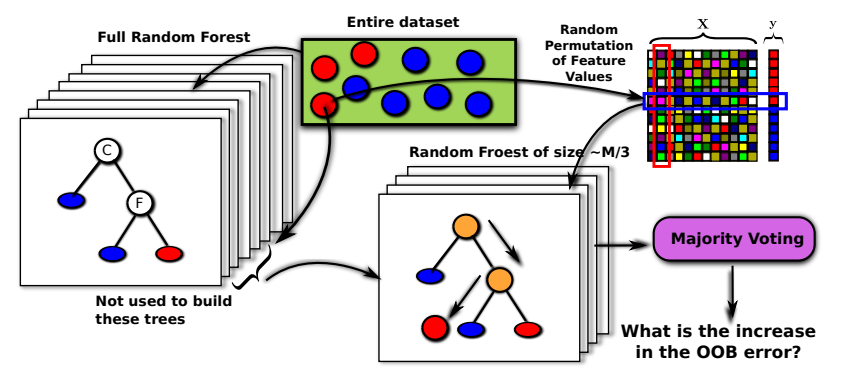
\includegraphics[width = 0.7\textwidth]{figs/random-forest-feature-selection.png}
\end{figure}

La ventaja es que se obtiene gratuitamente tras construir un random forest sobre los datos. Se pueden identificar los atributos que solo son relevantes cuando se consideran juntos, teniendo en cuenta las interacciones multivariantes. Además, devuelve una medida cuantitativa de la importancia (aumento del error), siendo relativamente barato de obtener. No obstante, puede sobreestimar la importancia de las variables predictoras correlacionadas debido a la preferencia de las variables predictoras correlacionadas en las primeras divisiones. También puede sobreestimar la importancia de variables categóricas con un gran número de categorías debido a su preferencia para dividir los datos.

\subsection{Sesgos en el proceso de selección de atributos}
Considerar un número reducido de características mejora la interpretabilidad, pero puede reducir el rendimiento de la predicción.

Muchos trabajos presentan estimaciones de rendimiento demasiado optimistas debido al uso de datos de prueba para llevar a cabo la selección de características.

Los datos de prueba no deben utilizarse en ninguna de las etapas de construcción del clasificador, incluidas la selección de características o la normalización de datos.

\begin{figure}[h]
\centering
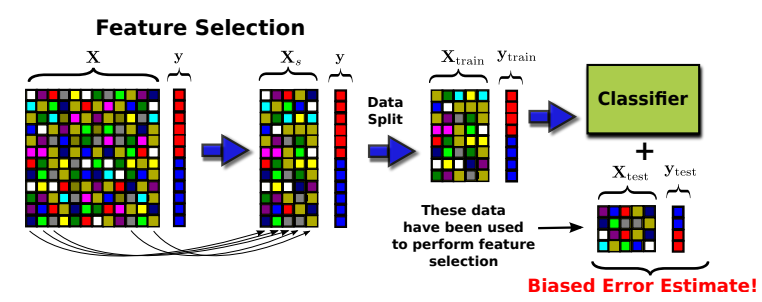
\includegraphics[width = 0.8\textwidth]{figs/feature-selection-bias.png}
\end{figure}

\subsection{Ejercicios}
\begin{enumerate}
\item \textit{En un conjunto de datos con 100.000 características y unos cientos de instancias, es demasiado costoso ejecutar Random Forest para la selección de características. Indique qué enfoques puede seguir para resolver este problema.}

Se podría hacer una preselección de atributos con variable ranking. De 100.000 podríamos quedarnos con 10.000 y después aplicar ya Random Forest.
\end{enumerate}

\subsection{Resumen}
\begin{itemize}
\item La selección de atributos puede utilizarse para identificar un pequeño conjunto de características más adecuadas para abordar una determinada tarea de clasificación.
\item Mejora la interpretabilidad del clasificador, simplifica la adquisición de datos y, en ocasiones, también mejora el rendimiento de la predicción.
\item La mayoría de las técnicas de selección de características pueden clasificarse en filtros, wrappers y métodos embebidos.
\item Los métodos de filtro son sencillos, rápidos y, la mayoría de las veces, suficientes para encontrar un buen conjunto de características para una tarea de clasificación concreta.
\item Existe un trade-off entre el número de características consideradas para la predicción y la precisión de la clasificación resultante.
\item Hay que tener cuidado para evitar sesgos optimistas en la estimación del rendimiento de predicción de un conjunto de características no utilizando datos de test para la selección de atributos.
\end{itemize}
